\chapter{Periodic Category}
\markboth{Periodic Category}{Periodic Category}

\begin{remark}[External dependencies of this chapter, and the order of reading]\label{rem:periodic_category_dependencies}
This chapter lifts the conclusions of the preceding chapters to the level of categories, and its exposition therefore cites several theorems from chapters that \textbf{come later} in the book. So that every step can be verified, these dependencies are collected here; each is given an explicit cross-reference at the point of use.
\begin{enumerate}[label=(\roman*)]
    \item \cref{thm:helmholtz} (the `Vector Analysis' chapter)---the Helmholtz decomposition;
    \item \cref{thm:noether_group_with_periodic_orbits} (the `Periodic Functions and Groups with Periodic Orbits' chapter)---Noether's theorem at the level of periodic functions;
    \item \cref{prop:commensurability_periodicity_parallel}, \cref{thm:intercalation_error_bound_parallel}, \cref{thm:continued_fraction_best_approx_parallel} (the `Discrete Sampling and Intercalation of Periodic Signals' chapter)---the commensurability parallel proposition, boundedness of the intercalation error, and continued-fraction optimality;
    \item \cref{thm:discrete_parseval_parallel} (the `Discrete Sampling and Intercalation of Periodic Signals' chapter), \cref{thm:parseval_fourier}, \cref{thm:intercalation_dft_leakage} (the `Harmonic Analysis' chapter)---the discrete and continuous Parseval identities, and the DFT leakage estimate.
\end{enumerate}
\textbf{Advice on reading}: the abstract conclusions of this chapter may be regarded as a \textbf{formal packaging} of concrete results already proved, and its proofs introduce no new substantial mathematics. On a first reading the chapter may be skipped and returned to after the `Harmonic Analysis' chapter, by which point every dependency is in place.
\end{remark}

\begin{remark}[Positioning of This Chapter]\label{rem:periodic_category_chapter_positioning}
Periodic categories constitute the highest level of unifying theory within periodic mathematics. This chapter unifies the mathematical structures built up in the preceding chapters---groups with periodic orbits, periodic functions, periodic convolution and periodic manifolds---within the language of category theory. Category theory provides the most abstract framework of expression for periodic mathematics, revealing the deep structural identity among different periodic structures.

This chapter first rigorously distinguishes the two basic concepts of \textbf{operator} and \textbf{functor}: an operator is a self-map within a single category, whilst a functor is a structure-preserving map between different categories. On this basis, the chapter establishes the complete theory of the \textbf{phase functor}: for any period $T$ and any phase $\theta \in [0, 2\pi)$, there exists a phase functor $\Phi_{\theta, T}$ that maps the translation-periodic category to itself. All phase functors form a parametrised family of functors.

The core content of this chapter:
\begin{enumerate}[label=(\arabic*)]
    \item \textbf{Rigorous distinction between operators and functors}: the essential differences between operators (Definition \ref{def:operator}) and functors (Definition \ref{def:functor}) in scope and in the preservation of structure.
    \item \textbf{Phase functors}: for any period $T$ and any phase $\theta$, the phase functor $\Phi_{\theta, T}$ (Definition \ref{def:phase_functor_general}) realises the phase translation of periodic structures.
    \item \textbf{Three basic periodic categories}: the translation-periodic category, the scaling-periodic category and the rotation-periodic category (Definitions \ref{def:translation_periodic_category} to \ref{def:scaling_periodic_category}).
    \item \textbf{Functors as category converters}: the logarithm functor effects the conversion from the scaling category to the translation category, and the Fourier functor effects the conversion from the translation category to the frequency-domain representation category.
    \item \textbf{Adjunction of the differential and integral operators}: $\mathcal{D} \dashv \mathcal{I}$.
    \item \textbf{Periodic convolution as a bifunctor}: periodic convolution is a bifunctor on the periodic category.
    \item \textbf{The observer as a functor}: the observer projects the periodic structures of the time system and the space system onto observable traces.
\end{enumerate}

\textbf{Guide to the seven themes of this chapter}: Translation---the translation-periodic category $\mathcal{C}_{\text{trans}}$ and the differential operator $\mathcal{D}$ ($0$-symmetry); Scaling---the scaling-periodic category and the logarithm/exponential functors ($1$-symmetry); Rotation---the rotation-periodic category and the phase functor ($i$-symmetry); Conservation---the conservation condition for adjoint operators ($\mathcal{I}\circ\mathcal{D}\cong\operatorname{id}$ requires the integral to vanish, corresponding to conservation of angular momentum); Symmetry---natural isomorphism and the adjoint duality $\mathcal{D}\dashv\mathcal{I}$; Closure---the mutual-inverse closure of the differential and integral operators, and the closure property of the periodic-convolution bifunctor; Period---the categorical formulation of periodic manifolds and the parametrisation of the phase functors.
\end{remark}

\begin{figure}[htbp]
\centering
\begin{tikzpicture}[
  font=\small,
  box/.style={draw, rounded corners, fill=blue!8, minimum width=2.6cm, minimum height=0.8cm, align=center},
  sub/.style={draw, rounded corners, fill=green!10, minimum width=2.4cm, minimum height=0.7cm, align=center, font=\footnotesize},
  arr/.style={->, thick, >=stealth}
]
  \node[box] (cat) {Foundations of category theory\\categories/functors/natural transformations};
  \node[box, right=1.0cm of cat] (phase) {Phase functors\\$\Phi_{\theta,T}$};
  \node[box, right=1.0cm of phase] (three) {Three periodic categories\\translation/scaling/rotation};
  \node[sub, below=1.0cm of cat] (diff) {Differential--integral adjunction\\$\mathcal D\dashv\mathcal I$};
  \node[sub, below=1.0cm of phase] (conv) {Periodic convolution bifunctor\\$\circledast$};
  \node[sub, below=1.0cm of three] (obs) {Observer functor\\$\mathcal P$};
  \node[box, fill=orange!12, below=1.0cm of $(diff)!0.5!(obs)$] (unify) {The categorical unification of periodic mathematics};
  \draw[arr] (cat) -- (phase);
  \draw[arr] (phase) -- (three);
  \draw[arr] (cat) -- (diff);
  \draw[arr] (phase) -- (conv);
  \draw[arr] (three) -- (obs);
  \draw[arr] (diff) -- (unify);
  \draw[arr] (conv) -- (unify);
  \draw[arr] (obs) -- (unify);
\end{tikzpicture}
\caption{Overview of the structure of this chapter: from the foundations of category theory, via the phase functor and the three periodic categories, to the differential--integral adjunction, the periodic convolution bifunctor and the observer functor, ultimately unified within the categorical framework of periodic mathematics.}
\label{fig:periodic_category_overview}
\end{figure}

\section{Foundations of Category Theory}\label{sec:category_theory_basics}

\begin{definition}[Category]\label{def:category}
A \textbf{category} $\mathcal{C}$ consists of the following data:
\begin{enumerate}[label=(\roman*)]
    \item A class of \textbf{objects} $\operatorname{Ob}(\mathcal{C})$.
    \item For any two objects $A, B \in \operatorname{Ob}(\mathcal{C})$, a set of \textbf{morphisms} $\operatorname{Hom}_{\mathcal{C}}(A, B)$.
    \item For any object $A$, an \textbf{identity morphism} $\operatorname{id}_A \in \operatorname{Hom}_{\mathcal{C}}(A, A)$.
    \item For any three objects $A, B, C$, a \textbf{composition} operation $\circ: \operatorname{Hom}_{\mathcal{C}}(B, C) \times \operatorname{Hom}_{\mathcal{C}}(A, B) \to \operatorname{Hom}_{\mathcal{C}}(A, C)$.
\end{enumerate}
satisfying the following axioms:
\begin{itemize}
    \item \textbf{Associativity}: for any $f: A \to B, g: B \to C, h: C \to D$, we have $h \circ (g \circ f) = (h \circ g) \circ f$.
    \item \textbf{Unit law}: for any $f: A \to B$, we have $f \circ \operatorname{id}_A = f = \operatorname{id}_B \circ f$.
\end{itemize}
\end{definition}

\begin{example}[Examples of Categories in Periodic Mathematics]\label{ex:category_instances}
\begin{itemize}
    \item \textbf{Category of sets} $\mathbf{Set}$: objects are sets, morphisms are functions.
    \item \textbf{Category of vector spaces} $\mathbf{Vect}_{\mathbb{C}}$: objects are complex vector spaces, morphisms are linear maps.
    \item \textbf{Category of groups} $\mathbf{Grp}$: objects are groups, morphisms are group homomorphisms.
    \item \textbf{Category of topological spaces} $\mathbf{Top}$: objects are topological spaces, morphisms are continuous maps.
    \item \textbf{Category of smooth manifolds} $\mathbf{Man}$: objects are smooth manifolds, morphisms are smooth maps.
\end{itemize}
\end{example}

\begin{figure}[htbp]
\centering
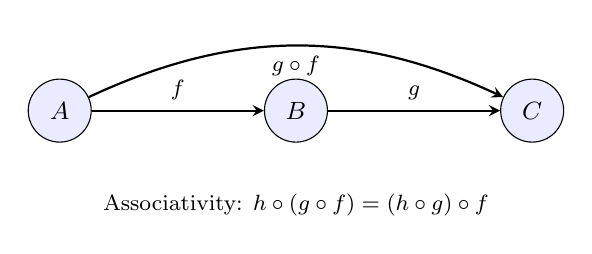
\begin{tikzpicture}[
  font=\small,
  obj/.style={circle, draw, fill=blue!8, minimum size=0.8cm, inner sep=2pt},
  arr/.style={->, thick, >=stealth}
]
  \node[obj] (A) at (0,0) {$A$};
  \node[obj] (B) at (3,0) {$B$};
  \node[obj] (C) at (6,0) {$C$};
  \draw[arr] (A) -- node[above, font=\footnotesize]{$f$} (B);
  \draw[arr] (B) -- node[above, font=\footnotesize]{$g$} (C);
  \draw[arr, bend left=25] (A) to node[below, font=\footnotesize]{$g\circ f$} (C);
  \node[font=\footnotesize] at (3,-1.2) {Associativity: $h\circ(g\circ f)=(h\circ g)\circ f$};
\end{tikzpicture}
\caption{The basic structure of a category: objects, morphisms and composition.}
\label{fig:category_structure}
\end{figure}

\section{Operators and Functors}\label{sec:operator_vs_functor}

\begin{definition}[Operator]\label{def:operator}
Let $\mathcal{C}$ be a category. An \textbf{operator} on $\mathcal{C}$ is a mapping $T: \operatorname{Ob}(\mathcal{C}) \to \operatorname{Ob}(\mathcal{C})$ such that for any morphism $f: A \to B$ there exists a morphism $T(f): T(A) \to T(B)$, and $T(\operatorname{id}_A) = \operatorname{id}_{T(A)}$, $T(g \circ f) = T(g) \circ T(f)$.

In other words, an operator is a \textbf{functor from a category to itself} (an endofunctor), namely $T: \mathcal{C} \to \mathcal{C}$. An operator preserves the internal structure of the category and does not change the category to which the objects belong.

In periodic mathematics, the differential operator $\mathcal{D}$ and the integral operator $\mathcal{I}$ are both operators (endofunctors) on the translation-periodic category $\mathcal{C}_{\text{trans}}$.
\end{definition}

\begin{definition}[Functor]\label{def:functor}
Let $\mathcal{C}$ and $\mathcal{D}$ be two categories. A \textbf{functor} $F: \mathcal{C} \to \mathcal{D}$ consists of the following data:
\begin{enumerate}[label=(\roman*)]
    \item For each object $A \in \operatorname{Ob}(\mathcal{C})$, an object $F(A) \in \operatorname{Ob}(\mathcal{D})$.
    \item For each morphism $f: A \to B$ (in $\mathcal{C}$), a morphism $F(f): F(A) \to F(B)$ (in $\mathcal{D}$).
\end{enumerate}
satisfying $F(\operatorname{id}_A) = \operatorname{id}_{F(A)}$ and $F(g \circ f) = F(g) \circ F(f)$.

If $F$ reverses the direction of morphisms (that is, $F(f): F(B) \to F(A)$), then $F$ is called a \textbf{contravariant functor}.
\end{definition}

\begin{remark}[Distinction between Operators and Functors]\label{rem:operator_vs_functor}
The essential difference between operators and functors lies in their \textbf{scope}:
\begin{itemize}
    \item An \textbf{operator} (endofunctor) $T: \mathcal{C} \to \mathcal{C}$ maps a category to \textbf{itself}, preserving the types of objects and morphisms. The differential operator $\mathcal{D}$ maps periodic functions to periodic functions and periodic morphisms to periodic morphisms---the periodic structure is preserved under the action of the operator.
    \item A \textbf{functor} $F: \mathcal{C} \to \mathcal{D}$ maps a category to \textbf{another category}, changing the types of objects and morphisms. The Fourier functor $\mathcal{F}: \mathcal{C}_{\text{trans}} \to \mathbf{Vect}_{\mathbb{C}}$ maps periodic functions to vectors of Fourier coefficients and periodic morphisms to linear maps---the periodic structure is `encoded' as an algebraic structure in the frequency domain.
\end{itemize}
From the perspective of periodic mathematics: an operator preserves the periodic type (a translation-periodic function remains translation-periodic after differentiation), whilst a functor converts the periodic type (a translation-periodic function becomes a discrete sequence in the frequency domain after the Fourier transform).
\end{remark}

\begin{figure}[htbp]
\centering
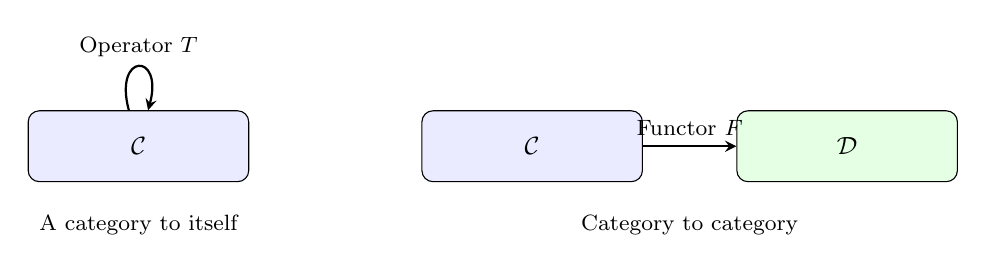
\begin{tikzpicture}[
  font=\small,
  cat/.style={draw, rounded corners, fill=blue!8, minimum width=2.8cm, minimum height=0.9cm, align=center},
  arr/.style={->, thick, >=stealth}
]
  % Operator
  \node[cat] (C1) at (0,0) {$\mathcal C$};
  \draw[arr] (C1) to[loop above] node[above, font=\footnotesize]{Operator $T$} (C1);
  \node[font=\footnotesize] at (0,-1.0) {A category to itself};
  % Functor
  \node[cat] (C2) at (5,0) {$\mathcal C$};
  \node[cat, fill=green!10] (D2) at (9,0) {$\mathcal D$};
  \draw[arr] (C2) -- node[above, font=\footnotesize]{Functor $F$} (D2);
  \node[font=\footnotesize] at (7,-1.0) {Category to category};
\end{tikzpicture}
\caption{A comparison of the scopes of operators (endofunctors) and functors: an operator does not change the category, whilst a functor maps between categories.}
\label{fig:operator_vs_functor}
\end{figure}

\section{The Phase Functor}\label{sec:phase_functor}

\begin{definition}[Phase Functor]\label{def:phase_functor_general}
Let $\mathcal{C}_{\text{trans}}$ be the translation-periodic category. For any period $T > 0$ and any phase $\theta \in [0, 2\pi)$, define the \textbf{phase functor} $\Phi_{\theta, T}: \mathcal{C}_{\text{trans}} \to \mathcal{C}_{\text{trans}}$ by:
\[
\Phi_{\theta, T}(f)(t) = e^{i\theta} \cdot f\!\left( t - \frac{\theta T}{2\pi} \right).
\]
That is, the phase functor shifts the periodic function $f$ in time by $\frac{\theta T}{2\pi}$ (the time offset corresponding to the phase $\theta$) and multiplies it by the phase factor $e^{i\theta}$.

The parameter space of the family of phase functors $\{\Phi_{\theta, T}\}_{\theta \in [0, 2\pi), T > 0}$ is $S^1 \times \mathbb{R}^+$.
\end{definition}

\begin{proposition}[Basic Properties of the Phase Functor]\label{prop:phase_functor_properties}
The phase functor $\Phi_{\theta, T}$ satisfies the following properties:
\begin{enumerate}[label=(\roman*)]
    \item \textbf{Functoriality}: $\Phi_{\theta, T}$ is an endofunctor (operator) on $\mathcal{C}_{\text{trans}}$.
    \item \textbf{Period preservation}: $\operatorname{Group}_{\mathrm{period}}(\Phi_{\theta, T}(f)) = \operatorname{Group}_{\mathrm{period}}(f)$---the phase functor does not change the period.
    \item \textbf{Composition law}: $\Phi_{\theta_1, T} \circ \Phi_{\theta_2, T} = \Phi_{\theta_1 + \theta_2, T}$ (modulo $2\pi$).
    \item \textbf{Identity element}: $\Phi_{0, T} = \operatorname{id}_{\mathcal{C}_{\text{trans}}}$ (pure time translation, with no phase factor).
    \item \textbf{Inverse element}: $\Phi_{\theta, T}^{-1} = \Phi_{-\theta, T} = \Phi_{2\pi - \theta, T}$.
    \item \textbf{Unitarity}: $\|\Phi_{\theta, T}(f)\| = \|f\|$ (the $L^2$ norm is preserved).
\end{enumerate}
\end{proposition}

\begin{proof}
(i) For any periodic morphism $h: f \to g$, $\Phi_{\theta, T}(h) = h$ (because the phase functor only shifts the time parameter and does not change the linear structure of the morphism). The preservation of identity morphisms and of composition is verified directly from the definition.

(ii) Time translation does not change the period: $f(t + T) = f(t)$ implies $f(t - \frac{\theta T}{2\pi} + T) = f(t - \frac{\theta T}{2\pi})$. Multiplication by $e^{i\theta}$ also does not change the period.

(iii)
\[
\Phi_{\theta_1, T}(\Phi_{\theta_2, T}(f))(t) = e^{i\theta_1} \Phi_{\theta_2, T}(f)\!\left( t - \tfrac{\theta_1 T}{2\pi} \right) = e^{i\theta_1} e^{i\theta_2} f\!\left( t - \tfrac{\theta_1 T}{2\pi} - \tfrac{\theta_2 T}{2\pi} \right) = \Phi_{\theta_1 + \theta_2, T}(f)(t).
\]

(iv) $\Phi_{0, T}(f)(t) = e^{i0} f(t - 0) = f(t)$.

(v) By (iii), $\Phi_{\theta, T} \circ \Phi_{-\theta, T} = \Phi_{0, T} = \operatorname{id}$.

(vi) $\|\Phi_{\theta, T}(f)\|^2 = \frac{1}{T}\int_0^T |e^{i\theta} f(t - \frac{\theta T}{2\pi})|^2 dt = \frac{1}{T}\int_0^T |f(t)|^2 dt = \|f\|^2$ (both time translation and multiplication by a unit complex number preserve the $L^2$ norm).
\end{proof}

\begin{theorem}[Group Structure of the Phase-Functor Family]\label{thm:phase_functor_group}
For a fixed period $T > 0$, the family of phase functors $\{\Phi_{\theta, T}\}_{\theta \in [0, 2\pi)}$ forms a group under functor composition, isomorphic to the circle group $U(1)$:
\[
\{\Phi_{\theta, T}\}_{\theta \in [0, 2\pi)} \cong U(1) \cong S^1.
\]
\end{theorem}

\begin{proof}
By (iii)(iv)(v) of Proposition \ref{prop:phase_functor_properties}, the set $\{\Phi_{\theta, T}\}$ is closed under composition, contains the identity element $\Phi_{0, T}$, and every element has an inverse $\Phi_{-\theta, T}$. Associativity is given by the associativity of function composition. The map $\theta \mapsto \Phi_{\theta, T}$ is a group isomorphism: $\Phi_{\theta_1 + \theta_2} = \Phi_{\theta_1} \circ \Phi_{\theta_2}$ (modulo $2\pi$), $\Phi_0 = \operatorname{id}$, $\Phi_{-\theta} = \Phi_\theta^{-1}$. Hence the family of phase functors is isomorphic to $U(1)$.
\end{proof}

\begin{corollary}[Functoriality of All Phases]\label{cor:all_phases_functorial}
For any period $T > 0$ and any phase $\theta \in [0, 2\pi)$, $\Phi_{\theta, T}$ is a functor (operator) on $\mathcal{C}_{\text{trans}}$. Consequently, \textbf{any phase of any period may serve as a functor}---phase is no longer an additional parameter of a function, but a structure-preserving map on a category.
\end{corollary}

\begin{proof}
By Theorem \ref{thm:phase_functor_group}, each $\Phi_{\theta, T}$ is an element of the group $U(1)$ and is therefore an invertible functor (an automorphism functor). Functoriality is guaranteed by Proposition \ref{prop:phase_functor_properties} (i).
\end{proof}

\begin{remark}[Phase Functor and the Discrete Phase Operator]\label{rem:phase_functor_discrete}
When the phase takes the discrete values $\theta_k = 2\pi k/T$ ($k = 0, 1, \dots, T-1$), the family of phase functors $\{\Phi_{\theta_k, T}\}_{k=0}^{T-1}$ is isomorphic to the cyclic group $C_T \cong \mathbb{Z}_T$. This is the functorial formulation of the discrete phase operator $\mathcal{O}_k^{(T)} = e^{i 2\pi k / T}$ (Definition \ref{def:discrete_phase_operator}) of the `Periodic Functions and Groups with Periodic Orbits' chapter. The continuous family of phase functors $U(1)$ is the continuous limit of the discrete family of phase operators $C_T$ ($T \to \infty$).
\end{remark}

\begin{example}[Concrete Action of the Phase Functor]\label{ex:phase_functor_action}
Take $T = 2\pi$ and $f(t) = \sin t$. For the phase $\theta = \pi/2$:
\[
\Phi_{\pi/2, 2\pi}(f)(t) = e^{i\pi/2} \sin\!\left( t - \frac{\pi/2 \cdot 2\pi}{2\pi} \right) = i \sin\!\left( t - \frac{\pi}{2} \right) = -i \cos t.
\]
That is, the phase functor $\Phi_{\pi/2, 2\pi}$ maps the sine function to the cosine function (multiplied by $-i$). This is precisely the standard operation of phase shifting in Fourier analysis.

For the phase $\theta = \pi$:
\[
\Phi_{\pi, 2\pi}(f)(t) = e^{i\pi} \sin(t - \pi) = -\sin(t - \pi) = \sin t = f(t).
\]
(Note that $\sin(t - \pi) = -\sin t$, so $e^{i\pi}\sin(t-\pi) = (-1)(-\sin t) = \sin t$.) Thus the functor of phase $\pi$ is the identity map on the sine function (because the sine function changes sign after a time translation by half a period, and multiplying by $-1$ restores its original form).
\end{example}

\begin{figure}[htbp]
\centering
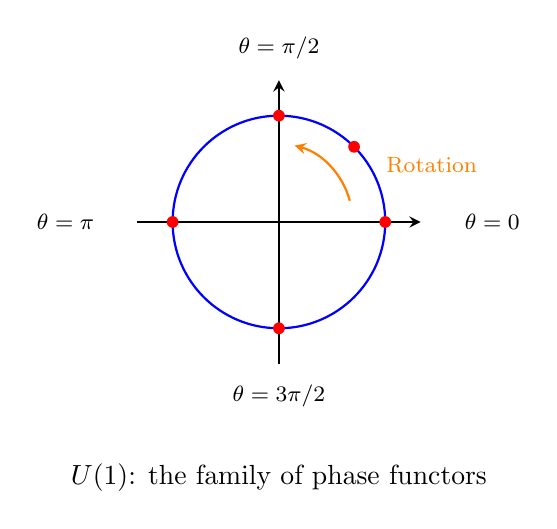
\begin{tikzpicture}[scale=0.9]

  \draw[->, thick, >=stealth] (-2,0) -- (2,0);
  \draw[->, thick, >=stealth] (0,-2) -- (0,2);

  \draw[thick, blue] (0,0) circle (1.5);

  \foreach \a in {0,45,90,180,270} {
    \node[circle, fill, red, inner sep=1.5pt] at (\a:1.5) {};
  }

  \node[font=\footnotesize, xshift=1cm] at (0:1.9) {$\theta=0$};
  \node[font=\footnotesize, yshift=0.5cm] at (90:1.9) {$\theta=\pi/2$};
  \node[font=\footnotesize, xshift=-1cm] at (180:1.9) {$\theta=\pi$};
  \node[font=\footnotesize, yshift=-0.5cm] at (270:1.9) {$\theta=3\pi/2$};

  \draw[->, thick, orange, >=stealth] (1.0,0.3) arc (15:75:1.1);
  \node[orange, font=\footnotesize, xshift=0.5cm] at (1.6,0.8) {Rotation};
  \node[yshift=-1cm] at (0,-2.5) {$U(1)$: the family of phase functors};
\end{tikzpicture}
\caption{The family of phase functors forms the circle group $U(1)$: the phase parameter $\theta$ varies continuously on the unit circle.}
\label{fig:phase_functor_U1}
\end{figure}

\section{Transformations and Evolution}\label{sec:transformation_evolution}

In category theory, changes of structure are described by two basic mechanisms: \textbf{transformation} (natural transformation) characterises comparisons between functors, whilst \textbf{evolution} (adjoint functors) characterises the mutual generation and forgetting between categories. This section establishes these two mechanisms and explains how they encode the birth and death of periodic structures.

\begin{definition}[Natural Transformation]\label{def:natural_transformation}
Let $F, G: \mathcal{C} \to \mathcal{D}$ be two parallel functors. A \textbf{natural transformation} $\eta: F \Rightarrow G$ consists of a family of morphisms $\{\eta_A: F(A) \to G(A)\}_{A \in \operatorname{Ob}(\mathcal{C})}$ such that for any $f: A \to B$ (in $\mathcal{C}$), the following diagram commutes:
\[
\begin{tikzcd}
F(A) \arrow[r, "F(f)"] \arrow[d, "\eta_A"'] & F(B) \arrow[d, "\eta_B"] \\
G(A) \arrow[r, "G(f)"'] & G(B)
\end{tikzcd}
\]
that is, $\eta_B \circ F(f) = G(f) \circ \eta_A$.
\end{definition}

\begin{definition}[Adjoint Functors]\label{def:adjoint_functor}
Let $F: \mathcal{C} \to \mathcal{D}$ and $G: \mathcal{D} \to \mathcal{C}$ be two functors. We say that $F$ is the \textbf{left adjoint} of $G$ (or that $G$ is the \textbf{right adjoint} of $F$), written $F \dashv G$, if there exists a natural isomorphism
\[
\operatorname{Hom}_{\mathcal{D}}(F(A), B) \cong \operatorname{Hom}_{\mathcal{C}}(A, G(B)),
\]
which is natural in $A \in \operatorname{Ob}(\mathcal{C})$ and $B \in \operatorname{Ob}(\mathcal{D})$.
\end{definition}

\begin{remark}[Adjoint Functors and the Periodic Lifecycle]\label{rem:adjunction_periodic_lifecycle}
In periodic mathematics, the adjoint pair $F \dashv G$ has a profound periodic-theoretic meaning: $F$ is the `generation' direction (symmetry breaking, the emergence of periodic structure), whilst $G$ is the `forgetting' direction (the degeneration of periodic structure). The adjoint pair $(F, G)$ constitutes a category-theoretic model of the birth and death of periodic structure---generation (the unit $\eta$ of the adjunction), evolution (composition of morphisms), and death (the degeneration of the counit $\varepsilon$ of the adjunction).

From the perspective of conservation laws, the \textbf{unit} $\eta: \operatorname{id}_{\mathcal{C}} \Rightarrow G \circ F$ of the adjoint pair $F \dashv G$ encodes the generation process `from aperiodic to periodic' (the establishment of conservation laws), whilst the \textbf{counit} $\varepsilon: F \circ G \Rightarrow \operatorname{id}_{\mathcal{D}}$ encodes the death process `from periodic to aperiodic' (the breaking of conservation laws).
\end{remark}

\begin{figure}[htbp]
\centering
\begin{tikzcd}[row sep=large, column sep=large]
\mathcal{C} \arrow[r, bend left=25, "F"] & \mathcal{D} \arrow[l, bend left=25, "G"]
\end{tikzcd}
\vspace{0.3cm}
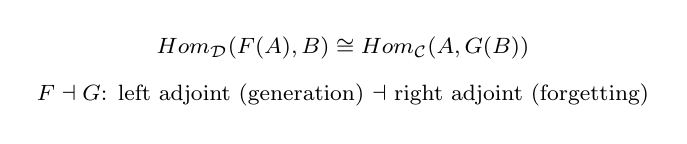
\begin{tikzpicture}[font=\footnotesize]
  \node at (0,0) {$\operatorname{Hom}_{\mathcal D}(F(A),B)\cong\operatorname{Hom}_{\mathcal C}(A,G(B))$};
  \node at (0,-0.6) {$F\dashv G$: left adjoint (generation) $\dashv$ right adjoint (forgetting)};
\end{tikzpicture}
\caption{The adjoint functor pair $F\dashv G$ and the natural isomorphism of Hom sets.}
\label{fig:adjoint_functor}
\end{figure}

\section{Fundamental Constructions of Periodic Categories}\label{sec:periodic_category_basic}

\subsection{Periodic Objects and Periodic Morphisms}

\begin{definition}[Periodic Object]\label{def:periodic_object}
Let $\mathcal{C}$ be a category and $G$ a group. A \textbf{$G$-periodic object} in $\mathcal{C}$ is a pair $(X, \rho)$, where $X \in \operatorname{Ob}(\mathcal{C})$ and $\rho: G \to \operatorname{Aut}_{\mathcal{C}}(X)$ is a group action of $G$ on $X$ (that is, $\rho(g): X \to X$ is an automorphism in $\mathcal{C}$, and $\rho(gh) = \rho(g) \circ \rho(h)$).

In periodic mathematics, $G$ is usually taken to be the translation group $\mathbb{R}$, the scaling group $\mathbb{R}^+$ or the rotation group $U(1)$.
\end{definition}

\begin{proposition}[Periodic Objects and Conservation Laws]\label{prop:periodic_object_conservation}
The group action $\rho$ of a $G$-periodic object $(X, \rho)$ implies a conservation structure on $X$: for any $g \in G$, $\rho(g)$ is an automorphism of $X$ that preserves all the category-theoretic structures of $X$. When $G$ is a continuous Lie group, Noether's theorem implies that each one-parameter subgroup of $G$ corresponds to a conserved quantity on $X$. Specifically:
\begin{enumerate}[label=(\roman*)]
    \item If $G = \mathbb{R}$ (translation group, $0$-symmetry), the conserved quantity is momentum/energy.
    \item If $G = U(1)$ (rotation group, $i$-symmetry), the conserved quantity is angular momentum.
    \item If $G = \mathbb{R}^+$ (scaling group, $1$-symmetry), the conserved quantity is the scale charge.
\end{enumerate}
\end{proposition}

\begin{proof}
In three steps, each labelled as to its nature.

\textbf{Step 1 (an unfolding of the definition, containing nothing additional)}. By Definition \ref{def:periodic_object}, $\rho$ is a group homomorphism $G \to \operatorname{Aut}_{\mathcal{C}}(X)$, that is, every $\rho(g)$ is an automorphism of $X$ in $\mathcal{C}$. An automorphism preserves, by definition, composition of morphisms and identity morphisms, and hence preserves all the categorical structure of $X$. This step merely restates the definition of an automorphism; it therefore establishes \textbf{invariance of structure}, and does not yet give any conserved quantity.

\textbf{Step 2 (the source of the conserved quantities)}. The conserved quantities come from a theorem at the concrete level: by \cref{thm:noether_group_with_periodic_orbits}, for each one-parameter subgroup $\{g_s\}_{s \in \mathbb{R}}$ of a continuous Lie group $G$, the family of actions $\rho(g_s)$ generates a conserved charge. Taking respectively
\[
\begin{aligned}
G = \mathbb{R} \;\Rightarrow\; &\text{translational charge (energy/momentum, symmetry centre } 0\text{)},\\
G = U(1) \;\Rightarrow\; &\text{rotational charge (angular momentum, symmetry centre } i\text{)},\\
G = \mathbb{R}^+ \;\Rightarrow\; &\text{scaling charge (scale charge, symmetry centre } 1\text{)}.
\end{aligned}
\]
gives exactly the three items listed in the proposition.

\textbf{Step 3 (the characterisation of the set of conserved quantities)}. The set of conserved quantities of the object $(X, \rho)$ is the union of the charges corresponding to all one-parameter subgroups. When $G$ is $\mathbb{R}$, $U(1)$ or $\mathbb{R}^+$, its one-parameter subgroups are respectively the translation family, the rotation family and the scaling family, so the three assertions hold one by one. This completes the proof.

\textbf{Note on dependencies}: Step 2 uses \cref{thm:noether_group_with_periodic_orbits}, a theorem that lies in the `Periodic Functions and Groups with Periodic Orbits' chapter, later than this one; see the declaration of dependencies at the head of this chapter, \cref{rem:periodic_category_dependencies}.
\end{proof}

\begin{definition}[Periodic Morphism]\label{def:periodic_morphism}
Let $(X, \rho)$ and $(Y, \sigma)$ be two $G$-periodic objects in $\mathcal{C}$. A \textbf{$G$-equivariant morphism} (or \textbf{periodic morphism}) $f: X \to Y$ satisfies, for any $g \in G$,
\[
f \circ \rho(g) = \sigma(g) \circ f.
\]
That is, $f$ commutes with the group action---$f$ preserves the periodic structure. All $G$-periodic objects together with the $G$-equivariant morphisms form the \textbf{periodic category} $\mathcal{C}^G$.
\end{definition}

\begin{theorem}[Conservation-Law Preservation of the Periodic Category]\label{thm:periodic_category_conservation}
Let $\mathcal{C}^G$ be the $G$-periodic category. Then:
\begin{enumerate}[label=(\roman*)]
    \item Every object $(X, \rho)$ in $\mathcal{C}^G$ carries the conserved quantities of $G$ (given by Noether's theorem).
    \item Every periodic morphism $f: (X, \rho) \to (Y, \sigma)$ in $\mathcal{C}^G$ preserves the conserved quantities.
    \item The isomorphism classes in $\mathcal{C}^G$ correspond to periodic objects with the same conserved-quantity structure.
\end{enumerate}
\end{theorem}

\begin{proof}
(i) Follows directly from Proposition \ref{prop:periodic_object_conservation}. (ii) The periodic morphism $f$ commutes with the group action: $f \circ \rho(g) = \sigma(g) \circ f$. Differentiating with respect to the one-parameter subgroup shows that $f$ maps the Noether charge of $X$ to the Noether charge of $Y$. (iii) Isomorphic periodic objects have isomorphic group actions and isomorphic spaces of conserved quantities.
\end{proof}

\begin{figure}[htbp]
\centering
\begin{tikzcd}[row sep=large, column sep=large]
X \arrow[r, "\rho(g)"] \arrow[d, "f"'] & X \arrow[d, "f"] \\
Y \arrow[r, "\sigma(g)"'] & Y
\end{tikzcd}
\caption{The equivariance condition for periodic morphisms: $f\circ\rho(g)=\sigma(g)\circ f$.}
\label{fig:periodic_morphism}
\end{figure}

\subsection{Three Fundamental Periodic Categories}

\begin{figure}[htbp]
\centering
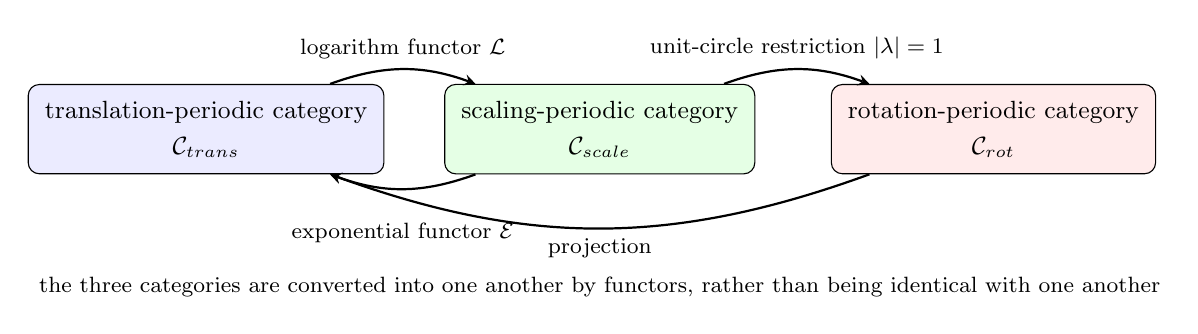
\begin{tikzpicture}[>=stealth,
  cat/.style={draw, rounded corners, align=center, font=\small, inner sep=6pt}]
  \node[cat, fill=blue!8, minimum width=3.0cm] (A) at (0,0) {translation-periodic category\\[2pt]$\mathcal{C}_{\text{trans}}$};
  \node[cat, fill=green!10, minimum width=3.0cm] (B) at (5.0,0) {scaling-periodic category\\[2pt]$\mathcal{C}_{\text{scale}}$};
  \node[cat, fill=red!8, minimum width=3.0cm] (C) at (10.0,0) {rotation-periodic category\\[2pt]$\mathcal{C}_{\text{rot}}$};
  \draw[->,thick] (A) to[bend left=20] node[above,font=\footnotesize]{logarithm functor $\mathcal{L}$} (B);
  \draw[->,thick] (B) to[bend left=20] node[below,font=\footnotesize,yshift=-0.3cm]{exponential functor $\mathcal{E}$} (A);
  \draw[->,thick] (B) to[bend left=20] node[above,font=\footnotesize]{unit-circle restriction $|\lambda|=1$} (C);
  \draw[->,thick] (C) to[bend left=20] node[below,font=\footnotesize]{projection} (A);
  \node[font=\footnotesize] at (5.0,-2.0) {the three categories are converted into one another by functors, rather than being identical with one another};
\end{tikzpicture}
\caption{The three basic periodic categories and their converting functors. The three kinds of generating transformation---translation, scaling and rotation---each correspond to a periodic category. The logarithm functor renders a multiplicative (scaling) structure additive (translational), with the exponential functor as its inverse; the unit-circle restriction separates the unit-modulus subcategory of the scaling category, giving the rotation category; and the projection sends the rotation category back to the translation category. This figure also makes plain that the three categories are not identical with one another, but are converted into one another by functors---which is precisely the reason why this chapter adopts the language of category theory.}
\label{fig:three_periodic_categories}
\end{figure}

\begin{definition}[Translation-Periodic Category]\label{def:translation_periodic_category}
Let $G = \mathbb{R}$ be the translation group (additive group). The objects of the \textbf{translation-periodic category} $\mathcal{C}_{\text{trans}}$ are periodic objects equipped with an $\mathbb{R}$-action---namely, translation-periodic functions $f: \mathbb{R} \to \mathbb{C}$ satisfying $f(t+T) = f(t)$. The morphisms are linear maps that commute with the translation action.
\end{definition}

\begin{definition}[Rotation-Periodic Category]\label{def:rotation_periodic_category}
Let $G = U(1)$ be the rotation group. The objects of the \textbf{rotation-periodic category} $\mathcal{C}_{\text{rot}}$ are periodic objects equipped with a $U(1)$-action---namely, rotation-periodic functions $f: \mathbb{C} \to \mathbb{C}$ satisfying $f(e^{i\theta}z) = f(z)$. The morphisms are linear maps that commute with the rotation action.
\end{definition}

\begin{definition}[Scaling-Periodic Category]\label{def:scaling_periodic_category}
Let $G = \mathbb{R}^+$ be the scaling group (multiplicative group). The objects of the \textbf{scaling-periodic category} $\mathcal{C}_{\text{scal}}$ are periodic objects equipped with an $\mathbb{R}^+$-action---namely, scaling-periodic functions $f: \mathbb{R}^+ \to \mathbb{C}$ satisfying $f(qx) = f(x)$. The morphisms are linear maps that commute with the scaling action.
\end{definition}

\begin{lemma}[Morphisms between Single-Frequency Circle Objects]\label{ch13_hom_frequency_lemma}
Let $\mathcal{C}_{\text{trans}}$ be the translation-periodic category, and let $f(t) = A\, e^{i(\omega_1 t + \varphi)}$, $g(t) = B\, e^{i(\omega_2 t + \psi)}$ be two single-frequency circle objects in it ($A, B > 0$, $\omega_1, \omega_2 \neq 0$). Then
\begin{enumerate}[label=(\roman*)]
    \item if $\omega_1 \neq \omega_2$, then $\operatorname{Hom}_{\mathcal{C}_{\text{trans}}}(f, g) = \{0\}$;
    \item if $\omega_1 = \omega_2 = \omega$, then
    \[
    \operatorname{Hom}_{\mathcal{C}_{\text{trans}}}(f, g) = \Big\{ c \cdot \tfrac{B}{A}\, e^{i(\psi - \varphi)} : c \in \mathbb{C} \Big\}.
    \]
\end{enumerate}
\end{lemma}

\begin{proof}
The action of the translation group on a single-frequency circle is scalar multiplication: $\rho_s(f)(t) = f(t+s) = e^{i\omega_1 s} f(t)$. The subspace spanned by $f$ is one-dimensional, so any morphism $\lambda: f \to g$ is scalar multiplication and must satisfy $\lambda f = c\, g$ ($c \in \mathbb{C}$), that is,
\[
\lambda A e^{i\varphi} e^{i\omega_1 t} = c B e^{i\psi} e^{i\omega_2 t} \qquad (\forall t).
\]
(i) If $\omega_1 \neq \omega_2$: evaluating at $t = 0$ gives $\lambda A e^{i\varphi} = c B e^{i\psi}$; differentiating with respect to $t$ and then evaluating at $t = 0$ gives $\lambda A e^{i\varphi} \omega_1 = c B e^{i\psi} \omega_2$. Dividing the two equations yields $\omega_1 = \omega_2$, a contradiction; hence $\lambda = 0$ and $c = 0$, that is, $\operatorname{Hom}(f, g) = \{0\}$.
(ii) If $\omega_1 = \omega_2 = \omega$: the equation above reduces to $\lambda A e^{i\varphi} = c B e^{i\psi}$, so $\lambda = c\,(B/A)\,e^{i(\psi-\varphi)}$ with $c$ arbitrary. Equivariance holds automatically.
\end{proof}

\begin{example}[Concrete Computation of a Single-Frequency Circle Morphism Set]\label{ch13_hom_set_example}
Take three single-frequency circle objects:
\[
f(t) = 3 e^{i(2t + \pi/6)}, \qquad g(t) = 2 e^{i(3t - \pi/4)}, \qquad h(t) = 5 e^{i(2t + \pi/3)}.
\]
(i) $\omega_f = 2 \neq 3 = \omega_g$, so by Lemma \ref{ch13_hom_frequency_lemma} (i), $\operatorname{Hom}(f, g) = \{0\}$.
(ii) $\omega_f = \omega_h = 2$, so by Lemma \ref{ch13_hom_frequency_lemma} (ii),
\[
\operatorname{Hom}(f, h) = \Big\{ c \cdot \tfrac{5}{3}\, e^{i(\pi/3 - \pi/6)} : c \in \mathbb{C} \Big\} = \Big\{ c \cdot \tfrac{5}{3}\, e^{i\pi/6} : c \in \mathbb{C} \Big\}.
\]
Taking $c = 1$ gives the standard morphism $\lambda = \tfrac{5}{3} e^{i\pi/6}$, and one verifies that $\lambda f(t) = \tfrac{5}{3} e^{i\pi/6} \cdot 3 e^{i(2t + \pi/6)} = 5 e^{i(2t + \pi/3)} = h(t)$.
(iii) Composition is preserved: take in addition $k(t) = 4 e^{i 2t}$. The standard morphism $h \to k$ is $\mu = \tfrac{4}{5} e^{-i\pi/3}$. The standard morphism $f \to k$ is $\nu = \tfrac{4}{3} e^{-i\pi/6}$; the composition $\mu \circ \lambda = \tfrac{4}{5} e^{-i\pi/3} \cdot \tfrac{5}{3} e^{i\pi/6} = \tfrac{4}{3} e^{-i\pi/6} = \nu$.
\end{example}

\begin{remark}[Amplitude and Phase Are Not Invariants of the Translation-Periodic Category]\label{ch13_amplitude_phase_remark}
Lemma \ref{ch13_hom_frequency_lemma} and Example \ref{ch13_hom_set_example} reveal a category-theoretic fact: in $\mathcal{C}_{\text{trans}}$, single-frequency circle objects of the same frequency are mutually isomorphic (any scalar morphism with $c \neq 0$ is an isomorphism), and the amplitude $A$ and the phase $\varphi$ do not enter the isomorphism invariants---they are `absorbed' by the morphism space. Amplitude and phase information is carried by additional structure at the level of functors (the phase functor $\Phi_{\theta, T}$, the similarity functor $\mathcal{S}^{(d)}$ and the tendency functor $\mathcal{T}^{(d)}$ are precisely the functors that extract this additional structure), and the skeleton of the category retains only the frequency (period) information.
\end{remark}

\begin{proposition}[Similarity Structure of the Translation-Periodic Category]\label{prop:translation_category_similarity}
In the translation-periodic category $\mathcal{C}_{\text{trans}}$, a non-trivial periodic morphism exists between two objects $f, g$ if and only if their Fourier expansions contain the same non-zero frequency. If $\operatorname{Group}_{\mathrm{period}}(f) \cap \operatorname{Group}_{\mathrm{period}}(g)$ is an infinite group (that is, the periods are commensurable), then their fundamental frequencies are commensurable, but they may have no common frequency component; a non-trivial morphism exists only when the frequency sets intersect.
\end{proposition}

\begin{proof}
At the level of Fourier modes (single-frequency circle components), by Lemma \ref{ch13_hom_frequency_lemma}: between components of the same frequency there exist non-zero scalar morphisms, whilst between components of different frequencies there is only the zero morphism. If the Fourier frequency sets of $f$ and $g$ have a non-zero intersection, then between the components corresponding to the intersecting frequencies there exist non-zero morphisms, and hence a non-trivial periodic morphism exists; if the frequency sets are disjoint, then every non-zero Fourier component has a distinct frequency, and the only frequency-preserving morphism left is the zero morphism.
\end{proof}

\begin{proposition}[Functorial Relations among the Three Periodic Categories]\label{prop:three_category_functors}
There exist natural functors among the three periodic categories:
\begin{enumerate}[label=(\roman*)]
    \item the \textbf{logarithm functor} $\mathcal{L}: \mathcal{C}_{\text{scal}} \to \mathcal{C}_{\text{trans}}$: maps the scaling-periodic function $f(x)$ to the translation-periodic function $g(t) = f(e^t)$.
    \item the \textbf{exponential functor} $\mathcal{E}: \mathcal{C}_{\text{trans}} \to \mathcal{C}_{\text{scal}}$: $\mathcal{E}(g)(x) = g(\ln x)$.
    \item the \textbf{Fourier functor} $\mathcal{F}: \mathcal{C}_{\text{trans}} \to \mathbf{Vect}_{\mathbb{C}}$: maps translation-periodic functions to their sequences of Fourier coefficients.
\end{enumerate}
\end{proposition}

\begin{proof}
(i) The logarithm functor $\mathcal{L}$: let $f \in \mathcal{C}_{\text{scal}}$ satisfy $f(qx) = f(x)$. Set $q = e^{\alpha}$ and $x = e^t$; then $g(t) = f(e^t)$ satisfies $g(t+\alpha) = g(t)$. Hence $g \in \mathcal{C}_{\text{trans}}$.

(ii) The exponential functor $\mathcal{E}$ is the inverse of $\mathcal{L}$: $\mathcal{E} \circ \mathcal{L} \cong \operatorname{id}_{\mathcal{C}_{\text{scal}}}$, $\mathcal{L} \circ \mathcal{E} \cong \operatorname{id}_{\mathcal{C}_{\text{trans}}}$.

(iii) The Fourier functor $\mathcal{F}$: the Fourier coefficients $\{c_n\}$ of the translation-periodic function $f(t) = \sum_n c_n e^{i 2\pi n t / T}$ form an object in $\mathbf{Vect}_{\mathbb{C}}$.
\end{proof}

\begin{corollary}[Adjointness of the Logarithm and Exponential Functors]\label{cor:grammar_adjunction}
The logarithm functor and the exponential functor form an adjoint pair:
\[
\mathcal{L} \dashv \mathcal{E}.
\]
\end{corollary}

\begin{proof}
Proposition \ref{prop:three_category_functors} (ii) has already proved that $\mathcal{E}\circ\mathcal{L} \cong \operatorname{id}_{\mathcal{C}_{\text{scal}}}$ and $\mathcal{L}\circ\mathcal{E} \cong \operatorname{id}_{\mathcal{C}_{\text{trans}}}$. For functors that are mutual pseudo-inverses one constructs the isomorphism of the adjunction (Definition \ref{def:adjoint_functor}); since both the unit and the counit are isomorphisms, it follows that $\mathcal{L} \dashv \mathcal{E}$.
\end{proof}

\section{Phase Functors, Similarity Functors and Tendency Functors}\label{sec:phase_similarity_tendency}

\subsection{The Phase-Extraction Functor}

\begin{definition}[Phase-Extraction Functor]\label{def:phase_extraction_functor}
Let $\mathcal{C}_{\text{trans}}$ be the translation-periodic category. The \textbf{phase-extraction functor} $\Phi: \mathcal{C}_{\text{trans}} \to \mathbf{Vect}_{\mathbb{C}}$ maps each periodic function to the vector space of its phase information:
\[
\Phi(f) = \{(\theta_n^{(f)}, A_n^{(f)}) \mid n \in \mathbb{Z}\},
\]
where $\theta_n^{(f)} = \arg(c_n^{(f)})$ is the phase of the $n$-th Fourier component and $A_n^{(f)} = |c_n^{(f)}|$ is the amplitude of the $n$-th Fourier component.
\end{definition}

\begin{remark}[Distinction between the Phase-Extraction Functor and the Phase Functor]\label{rem:phase_extraction_vs_phase_functor}
Note the distinction between two different concepts:
\begin{itemize}
    \item the \textbf{phase functor} $\Phi_{\theta, T}$ (Definition \ref{def:phase_functor_general}): parameterised by the phase $\theta$, it is an \textbf{operator} (endofunctor) on $\mathcal{C}_{\text{trans}}$ that maps a function $f$ to a function that is time-shifted and multiplied by a phase factor.
    \item the \textbf{phase-extraction functor} $\Phi$ (Definition \ref{def:phase_extraction_functor}): it extracts the phase information of a function, and is a \textbf{functor} (across categories) $\mathcal{C}_{\text{trans}} \to \mathbf{Vect}_{\mathbb{C}}$ that maps a function to the vector space of phase--amplitude pairs.
\end{itemize}
\end{remark}

\begin{proposition}[Relation between the Phase-Extraction Functor and the Differential Operator]\label{prop:phase_extraction_differential}
The phase-extraction functor $\Phi$ and the differential operator $\mathcal{D}$ satisfy:
\[
\Phi(\mathcal{D}f) = \{(\theta_n^{(f)} + \pi/2, |n\omega_0| \cdot A_n^{(f)}) \mid n \in \mathbb{Z}\}.
\]
That is, differentiation increases the phase of each Fourier component by $\pi/2$ and multiplies its amplitude by $|n\omega_0|$.
\end{proposition}

\begin{proof}
By the differentiation property of Fourier series: $f'(t) = \sum_n i n \omega_0 c_n e^{i n \omega_0 t}$. The coefficient $i n \omega_0 c_n = |n\omega_0| \cdot |c_n| \cdot e^{i(\theta_n + \pi/2)}$ (because $i = e^{i\pi/2}$).
\end{proof}

\subsection{Similarity Functors and Tendency Functors}

\begin{definition}[Similarity Functor]\label{def:similarity_functor}
Let $\mathcal{C}_{\text{trans}}$ be the translation-periodic category. For the $d$-th dimension ($d = 1,\dots,12$), the \textbf{similarity functor} $\mathcal{S}^{(d)}: \mathcal{C}_{\text{trans}} \times \mathcal{C}_{\text{trans}} \to \mathbf{Set}$ maps two periodic functions to the set of their directional relations under the $d$-th kind of similarity:
\[
\mathcal{S}^{(d)}(f, g) = \{\operatorname{Similarity}^{(d)}(\theta_n^{(f)}, \theta_m^{(g)}) \mid n, m \in \mathbb{Z}\}.
\]
The similarity functor is determined solely by directional relations and contains no scale information.
\end{definition}

\begin{definition}[Tendency Functor]\label{def:tendency_functor}
Let $\mathcal{C}_{\text{trans}}$ be the translation-periodic category. For the $d$-th dimension ($d = 1,\dots,12$), the \textbf{tendency functor} $\mathcal{T}^{(d)}: \mathcal{C}_{\text{trans}} \times \mathcal{C}_{\text{trans}} \to \mathbf{Set}$ maps two periodic functions to the set of their combined directional-scale relations under the $d$-th kind of tendency:
\[
\mathcal{T}^{(d)}(f, g) = \{A_n^{(f)} A_m^{(g)} \cdot \operatorname{Similarity}^{(d)}(\theta_n^{(f)}, \theta_m^{(g)}) \mid n, m \in \mathbb{Z}\}.
\]
\end{definition}

\begin{proposition}[Relation between the Similarity and Tendency Functors]\label{prop:similarity_tendency_functor_relation}
The tendency functor $\mathcal{T}^{(d)}$ is the `scaled' version of the similarity functor $\mathcal{S}^{(d)}$:
\[
\mathcal{T}^{(d)}(f, g) = \mathcal{A}(f) \otimes \mathcal{A}(g) \cdot \mathcal{S}^{(d)}(f, g),
\]
where $\mathcal{A}(f) = \{A_n^{(f)}\}_{n \in \mathbb{Z}}$ is the amplitude-extraction map.
\end{proposition}

\begin{proof}
This follows immediately by checking element by element against Definitions \ref{def:similarity_functor} and \ref{def:tendency_functor}.
\end{proof}

\begin{proposition}[Conservation Laws of the Similarity and Tendency Functors]
\label{prop:similarity_tendency_conservation}
\begin{enumerate}[label=(\roman*)]
    \item \textbf{Rotational invariance of the similarity functor}:
    \[
    \mathcal{S}^{(d)}(e^{i\phi} f, e^{i\phi} g)
    = \mathcal{S}^{(d)}(f, g).
    \]

    \item \textbf{Scale covariance of the tendency functor}:
    \[
    \mathcal{T}^{(d)}(\lambda f, \lambda g)
    = \lambda^2 \cdot \mathcal{T}^{(d)}(f, g).
    \]

    \item \textbf{Parseval identity of the tendency functor}:
    \[
    \mathcal{T}^{(1)}(f, f) = \sum_n |c_n^{(f)}|^2.
    \]
\end{enumerate}
\end{proposition}

\begin{proof}
(i) The rotation factor increases all phases by $\phi$, and similarity depends only on the phase difference. (ii) The scaling factor multiplies all amplitudes by $\lambda$. (iii) By the Parseval identity (Theorem \ref{thm:parseval_fourier} of the `Harmonic Analysis' chapter).
\end{proof}

\begin{example}[Similarity and Tendency Functor Matrices on $C_4$]\label{ch13_c4_similarity_example}
Take the $C_4$ phase operator $\mathcal{O}_k^{(4)} = e^{i k\pi/2}$ ($k = 0,1,2,3$) and construct two sequences of period $4$
\[
f = (1,\, i,\, -1,\, -i), \qquad g = (i,\, -1,\, -i,\, 1),
\]
that is, $f_n = e^{i n\pi/2}$, $g_m = e^{i (m+1)\pi/2}$. The component-pair matrices of the basic difference-angle similarity functor $\mathcal{S}^{(1)}$ (cosine) and $\mathcal{S}^{(2)}$ (sine) are
\[
\mathcal{S}^{(1)}(f, g) =
\begin{pmatrix}
0 & -1 & 0 & 1 \\
1 & 0 & -1 & 0 \\
0 & 1 & 0 & -1 \\
-1 & 0 & 1 & 0
\end{pmatrix}, \qquad
\mathcal{S}^{(2)}(f, g) =
\begin{pmatrix}
-1 & 0 & 1 & 0 \\
0 & -1 & 0 & 1 \\
1 & 0 & -1 & 0 \\
0 & 1 & 0 & -1
\end{pmatrix}.
\]
At each position there is exactly one non-zero entry (with value $\pm 1$), and $\big(\mathcal{S}^{(1)}_{n,m}\big)^2 + \big(\mathcal{S}^{(2)}_{n,m}\big)^2 = 1$ holds for all $16$ positions. Since all the amplitudes are $A_n = B_m = 1$, the tendency functor coincides with the similarity functor: $\mathcal{T}^{(d)}(f, g) = \mathcal{S}^{(d)}(f, g)$.
\end{example}

\section{Category-Theoretic Formulations of Differentiation, Integration and Convolution}\label{sec:diff_int_conv_category}

\subsection{Differential and Integral Operators}

\begin{definition}[Differential Operator]\label{def:differential_operator}
The \textbf{differential operator} $\mathcal{D}: \mathcal{C}_{\text{trans}} \to \mathcal{C}_{\text{trans}}$ is defined as pointwise differentiation of periodic functions:
\[
\mathcal{D}(f) = f'.
\]
The differential operator is an operator (endofunctor) on $\mathcal{C}_{\text{trans}}$.
\end{definition}

\begin{definition}[Integral Operator]\label{def:integral_operator}
The \textbf{integral operator} $\mathcal{I}: \mathcal{C}_{\text{trans}} \to \mathcal{C}_{\text{trans}}$ is defined as pointwise integration of periodic functions (with the mean subtracted so as to ensure periodicity):
\[
\mathcal{I}(f)(t) = \int_0^t (f(\tau) - \bar{f}) d\tau, \quad \text{where } \bar{f} = \frac{1}{T}\int_0^T f(\tau) d\tau.
\]
The integral operator is an operator (endofunctor) on $\mathcal{C}_{\text{trans}}$.
\end{definition}

\begin{lemma}[Differentiation Does Not Change the Group with Periodic Orbits]\label{ch13_derivative_period_lemma}
Let $f$ be a non-zero continuous $T$-periodic function whose minimal positive period is $T > 0$. Then $\operatorname{Group}_{\mathrm{period}}(f') = \operatorname{Group}_{\mathrm{period}}(f)$: differentiation preserves the group with periodic orbits.
\end{lemma}

\begin{proof}
First we prove $\operatorname{Group}_{\mathrm{period}}(f') \supseteq \operatorname{Group}_{\mathrm{period}}(f)$: $f'$ has period $T$. Next we prove $\operatorname{Group}_{\mathrm{period}}(f') \subseteq \operatorname{Group}_{\mathrm{period}}(f)$: let $\tau \in \operatorname{Group}_{\mathrm{period}}(f')$ and set $g(t) = f(t+\tau) - f(t)$; then $g'(t) = 0$, so $g$ is a constant function: $f(t+\tau) = f(t) + c$. If $c \neq 0$, then $f(t + n\tau) = f(t) + nc$ is unbounded---contradicting the boundedness of a continuous periodic function. Hence $c = 0$, that is, $\tau \in \operatorname{Group}_{\mathrm{period}}(f)$.
\end{proof}

\begin{theorem}[Adjointness of Differentiation and Integration]\label{thm:diff_int_adjunction}
On the translation-periodic category $\mathcal{C}_{\text{trans}}$, the differential operator $\mathcal{D}$ and the integral operator $\mathcal{I}$ form an adjoint pair:
\[
\mathcal{D} \dashv \mathcal{I}.
\]
\end{theorem}

\begin{proof}
By the fundamental theorem of calculus of the `Functions and Limits' chapter, $(\mathcal{I} \circ \mathcal{D})(f) = f - \bar{f}$ and $(\mathcal{D} \circ \mathcal{I})(f) = f - \bar{f}$. On the space of zero-mean periodic functions, $\mathcal{D}$ and $\mathcal{I}$ are mutually inverse maps. On the general space of periodic functions, the two form an adjoint pair, and the natural isomorphism of the adjunction is given by the formula for integration by parts.
\end{proof}

\begin{lemma}[Differentiation and Integration Are Strict Inverses on the Quotient Category]\label{ch13_diff_int_inverse_lemma}
Let $\mathcal{D}, \mathcal{I}$ be the differential and integral operators of Definitions \ref{def:differential_operator} and \ref{def:integral_operator}. Then:
\begin{enumerate}[label=(\roman*)]
    \item $(\mathcal{D} \circ \mathcal{I})(f) = f - \bar{f}$, $(\mathcal{I} \circ \mathcal{D})(f) = f - f(0)$.
    \item On the quotient category (modulo constants) of zero-mean periodic functions, $\mathcal{D} \circ \mathcal{I} \equiv \operatorname{id}$ and $\mathcal{I} \circ \mathcal{D} \equiv \operatorname{id}$.
\end{enumerate}
\end{lemma}

\begin{proof}
(i) By Definition \ref{def:integral_operator}, $\mathcal{I}f = \int_0^t (f - \bar{f})$, and differentiating gives $(\mathcal{I}f)' = f - \bar{f}$. For the second formula: $\mathcal{D}f = f'$ and $\overline{f'} = 0$, so $(\mathcal{I}\circ\mathcal{D})(f)(t) = \int_0^t f'(\tau)d\tau = f(t) - f(0)$.
(ii) On the zero-mean subcategory $\bar{f} = 0$, and by (i) we obtain $\mathcal{D}\mathcal{I}f = f$ and $\mathcal{I}\mathcal{D}f = f - f(0) \sim f$ (modulo constants).
\end{proof}

\begin{example}[Numerical Verification of the Adjoint Inverses]\label{ch13_adjunction_numeric_example}
(i) Take $f(t) = \sin(2\pi t/3)$ ($T = 3$). Then $\bar{f} = 0$ and $f(0) = 0$:
\[
(\mathcal{D}\circ\mathcal{I})f = f, \qquad (\mathcal{I}\circ\mathcal{D})f = f.
\]
(ii) Take $g(t) = \cos(2\pi t/3)$ ($T = 3$). Then $\bar{g} = 0$ but $g(0) = 1$:
\[
(\mathcal{D}\circ\mathcal{I})g = g, \qquad (\mathcal{I}\circ\mathcal{D})g(t) = g(t) - 1.
\]
In the sense of the quotient category (modulo constants), $\cos(2\pi t/3) - 1 \sim \cos(2\pi t/3)$, and the two are mutual inverses throughout.
\end{example}

\begin{corollary}[Differentiation--Integration Adjointness and Conservation Laws]\label{cor:diff_int_conservation}
The validity of the adjoint pair $\mathcal{D} \dashv \mathcal{I}$ depends on the conservation structure of periodic functions:
\begin{enumerate}[label=(\roman*)]
    \item $\mathcal{D} \circ \mathcal{I} \cong \operatorname{id}$ requires $\bar{f} = 0$---the zero-mean condition (conservation of momentum).
    \item $\mathcal{I} \circ \mathcal{D} \cong \operatorname{id}$ (in the quotient-category sense) requires the total circulation to vanish (conservation of angular momentum).
    \item The preservation of the $L^2$ norm under differentiation and integration is given by the Parseval identity (conservation of the scale charge).
\end{enumerate}
\end{corollary}

\begin{proof}
Follows directly from Lemma \ref{ch13_diff_int_inverse_lemma}.
\end{proof}

\begin{figure}[htbp]
\centering
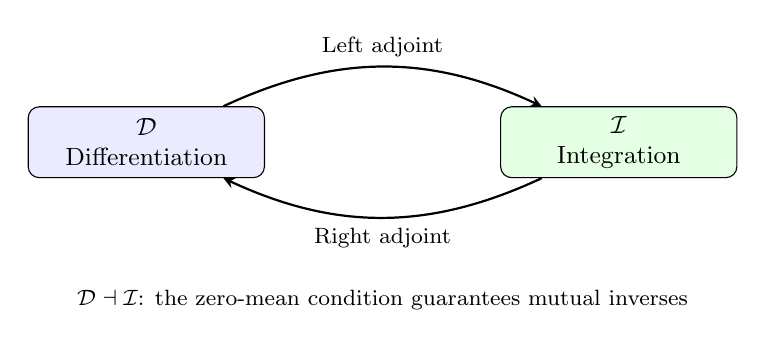
\begin{tikzpicture}[font=\small, arr/.style={->, thick, >=stealth}]
  \node[draw, rounded corners, fill=blue!8, minimum width=3cm, minimum height=0.9cm, align=center] (D) at (0,0) {$\mathcal D$\\Differentiation};
  \node[draw, rounded corners, fill=green!10, minimum width=3cm, minimum height=0.9cm, align=center] (I) at (6,0) {$\mathcal I$\\Integration};
  \draw[arr, bend left=25] (D) to node[above, font=\footnotesize]{Left adjoint} (I);
  \draw[arr, bend left=25] (I) to node[below, font=\footnotesize]{Right adjoint} (D);
  \node[font=\footnotesize, yshift=-0.5cm] at (3,-1.5) {$\mathcal D\dashv\mathcal I$: the zero-mean condition guarantees mutual inverses};
\end{tikzpicture}
\caption{The adjoint pair of the differential and integral operators: $\mathcal D\dashv\mathcal I$.}
\label{fig:diff_int_adjunction}
\end{figure}

\subsection{Convolution as a Bifunctor}

\begin{definition}[Convolution Bifunctor]\label{def:convolution_bifunctor}
The \textbf{convolution bifunctor} $*: \mathcal{C}_{\text{trans}} \times \mathcal{C}_{\text{trans}} \to \mathcal{C}_{\text{trans}}$ is defined as the cyclic convolution of periodic functions:
\[
(f * g)(t) = \frac{1}{T} \int_0^T f(\tau) g(t-\tau) d\tau.
\]
\end{definition}

\begin{proposition}[The Convolution Bifunctor and the Calculus]\label{prop:convolution_diff_int}
\begin{enumerate}[label=(\roman*)]
    \item $\mathcal{D}(f * g) = (\mathcal{D}f) * g = f * (\mathcal{D}g)$.
    \item $\mathcal{I}(f * g) = (\mathcal{I}f) * g = f * (\mathcal{I}g)$ (in the quotient-category sense).
    \item $(f * \mathcal{I}g) = \mathcal{I}(f * g) = (\mathcal{I}f * g)$ (in the quotient-category sense).
\end{enumerate}
\end{proposition}

\begin{proof}
(i) Differentiate under the integral sign. (ii)(iii) Follow from Lemma \ref{ch13_diff_int_inverse_lemma} and the commutativity of cyclic convolution.
\end{proof}

\section{Category-Theoretic Formulation of Periodic Convolution}\label{sec:periodic_convolution_category}

\begin{definition}[Periodic-Convolution Bifunctor]\label{def:periodic_convolution_bifunctor}
The \textbf{periodic-convolution bifunctor} $\circledast: \mathcal{C}_{\text{trans}} \times \mathcal{C}_{\text{trans}} \to \mathcal{C}_{\text{trans}}$ takes the four parameters of amplitude, frequency, phase and period as its operators, retaining the interaction of all frequency pairs and all period pairs. Its definition at the level of objects is: for any two translation-periodic functions $f, g$, the Fourier coefficients of their periodic convolution $(f \circledast g)$ are given by the products over all frequency pairs:
\[
c_{n,m}^{(f \circledast g)} = c_n^{(f)} \cdot c_m^{(g)}, \qquad \forall n, m \in \mathbb{Z}.
\]
The periodic-convolution bifunctor is a generalisation of the traditional convolution bifunctor (Definition \ref{def:convolution_bifunctor}): the traditional convolution retains only the diagonal terms $n=m$, whereas the periodic convolution retains the phase pairs for all $n,m$.
\end{definition}

\begin{theorem}[Functoriality of Periodic Convolution]\label{thm:periodic_convolution_functoriality}
The first statement of this same set of functoriality conditions is given in Chapter~\ref{chap:series_conv}, in \cref{subsec:periodic_convolution_series}, at \cref{thm:periodic_convolution_functoriality_series}; the present statement is its restatement in the language of category theory.
The periodic-convolution bifunctor $\circledast$ satisfies the following functoriality conditions:
\begin{enumerate}[label=(\roman*)]
    \item \textbf{Preservation of identity morphisms}: $\operatorname{id}_f \circledast \operatorname{id}_g = \operatorname{id}_{f \circledast g}$.
    \item \textbf{Preservation of composition}: $(h_2 \circ h_1) \circledast (k_2 \circ k_1) = (h_2 \circledast k_2) \circ (h_1 \circledast k_1)$.
    \item \textbf{Compatibility with the similarity functor}: $\mathcal{S}^{(d)}(f \circledast g, h) \cong \mathcal{S}^{(d)}(f, h) \otimes \mathcal{S}^{(d)}(g, h)$.
    \item \textbf{Compatibility with the tendency functor}: $\mathcal{T}^{(d)}(f \circledast g, h) \cong \mathcal{T}^{(d)}(f, h) \otimes \mathcal{T}^{(d)}(g, h)$.
\end{enumerate}
\end{theorem}

\begin{proof}
(i)-(ii) Are guaranteed by the linearity of periodic convolution and the functoriality of the Fourier transform. (iii)-(iv) Are verified directly from the frequency-domain representation of periodic convolution (the outer product $\mathbf{c}_f \otimes \mathbf{c}_g$) and the definitions of similarity/tendency.
\end{proof}

\begin{figure}[htbp]
\centering
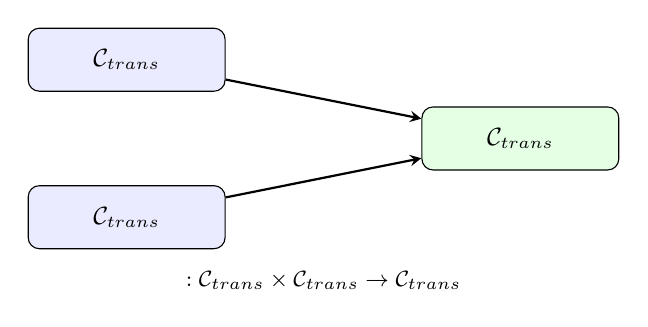
\begin{tikzpicture}[font=\small, arr/.style={->, thick, >=stealth}]
  % Bifunctor
  \node[draw, rounded corners, fill=blue!8, minimum width=2.5cm, minimum height=0.8cm] (A) at (0,1) {$\mathcal C_{\text{trans}}$};
  \node[draw, rounded corners, fill=blue!8, minimum width=2.5cm, minimum height=0.8cm] (B) at (0,-1) {$\mathcal C_{\text{trans}}$};
  \node[draw, rounded corners, fill=green!10, minimum width=2.5cm, minimum height=0.8cm] (C) at (5,0) {$\mathcal C_{\text{trans}}$};
  \draw[arr] (A) -- node[above, font=\footnotesize]{$\circledast$} (C);
  \draw[arr] (B) -- (C);
  \node[font=\footnotesize] at (2.5,-1.8) {$\circledast:\mathcal C_{\text{trans}}\times\mathcal C_{\text{trans}}\to\mathcal C_{\text{trans}}$};
\end{tikzpicture}
\caption{The periodic-convolution bifunctor: a two-variable input, retaining the interaction of all frequency pairs.}
\label{fig:periodic_convolution_bifunctor}
\end{figure}

\section{Category-Theoretic Formulation of Periodic Manifolds}\label{sec:periodic_manifold_category}

\begin{definition}[Discrete-Lattice Category]\label{def:discrete_lattice_category}
Let $\mathcal{L}$ be a discrete spacetime lattice (Definition \ref{def:discrete_spacetime_lattice} of the `Periodic Manifold' chapter). The \textbf{discrete-lattice category} $\mathbf{Latt}$ is defined as follows:
\begin{enumerate}[label=(\roman*)]
    \item \textbf{Objects}: potential vector fields on the lattice $\mathbf{V}: \mathcal{L} \to \mathbb{R}^d$ (or $\mathbb{C}^d$).
    \item \textbf{Morphisms}: discrete translations between lattice sites $\mathcal{T}_{\mathbf{m}}$, discrete rotations $\mathcal{R}_\theta$, discrete scalings $\mathcal{S}_\alpha$, and their compositions.
\end{enumerate}
\end{definition}

\begin{definition}[Continuum-Limit Functor]\label{def:continuum_limit_functor}
The \textbf{continuum-limit functor} $\mathcal{C}_{\infty}: \mathbf{Latt} \to \mathbf{Man}$ maps a discrete-lattice manifold to its continuum limit:
\[
\mathcal{C}_{\infty}(\mathcal{L}) = \lim_{\Delta x \to 0} \mathcal{L}_{\Delta x}.
\]
\end{definition}

\begin{proposition}[Continuum-Limit Functor and Adjointness]\label{prop:continuum_limit_adjunction}
The continuum-limit functor $\mathcal{C}_{\infty}$ and the discretisation functor $\mathcal{D}: \mathbf{Man} \to \mathbf{Latt}$ form an adjoint pair:
\[
\mathcal{D} \dashv \mathcal{C}_{\infty}.
\]
\end{proposition}

\begin{proof}
We construct the natural bijection of the adjunction (Definition \ref{def:adjoint_functor}):
\[
\operatorname{Hom}_{\mathbf{Latt}}(\mathcal{D}M, L) \cong \operatorname{Hom}_{\mathbf{Man}}(M, \mathcal{C}_{\infty}L).
\]
From right to left: a continuous map $\varphi: M \to \mathcal{C}_{\infty}L$, restricted to the discretised lattice, gives a lattice morphism. From left to right: a lattice morphism, once embedded in the limit, extends uniquely to a continuous map by the unique determinacy of the continuum limit (Theorem \ref{thm:continuum_limit_full} of the `Periodic Manifold' chapter). The two maps are mutually inverse, so $\mathcal{D} \dashv \mathcal{C}_{\infty}$.
\end{proof}

\begin{remark}[Interface with the `Periodic Manifold' Chapter]\label{ch13_periodic_manifold_interface_remark}
The family of morphisms $\{\mathcal{T}_{\mathbf{m}}, \mathcal{R}_\theta, \mathcal{S}_\alpha\}$ of the discrete-lattice category $\mathbf{Latt}$ corresponds to the three fundamental operations of the `Periodic Manifold' chapter, and the continuum-limit functor $\mathcal{C}_{\infty}$ is the functorialisation of the continuous-limit theorem of that chapter (Theorem \ref{thm:continuum_limit_full}). Discrete curvature and Wilson loops correspond to closed-loop morphisms in $\mathbf{Latt}$.
\end{remark}

\section{Intercalation Functor: Categorical Correction for Incommensurable Periods}\label{sec:intercalation_functor}

\begin{remark}[Positioning of This Section]\label{rem:intercalation_functor_positioning}
The preceding section, `Category-Theoretic Formulation of Periodic Manifolds', established the continuum-limit functor $\mathcal{C}_\infty:\mathbf{Latt}\to\mathbf{Man}$ and its left adjoint---the discretisation functor $\mathcal{D}:\mathbf{Man}\to\mathbf{Latt}$. However, when the continuous period $T_F$ and the sampling step $\Delta x$ are incommensurable (that is, the ideal period ratio $\rho = T_F/\Delta x \notin \mathbb{Q}$), the uniform sampling sequence no longer has a strict integer period, and the discretisation functor $\mathcal{D}$ fails to preserve the periodic structure in this situation---this is a logical gap in the categorical chain.

This section introduces the \textbf{intercalation functor} $\mathcal{R}:\mathcal{C}_{\text{cont}}\to\mathcal{C}_{\text{trans}}$ to repair this gap. Its core idea is to approximate the ideal period ratio $\rho$ by an integer sequence $\{N_m\}$, so that the cumulative sampling error is bounded. At the categorical level the intercalation functor carries three structures---the \textbf{intercalation object} (Definition \ref{def:intercalation_object}), the \textbf{functoriality of the intercalation sequence} (Theorem \ref{thm:intercalation_functoriality}) and the \textbf{commutation law with the continuum-limit functor} (Theorem \ref{thm:intercalation_continuum_commutation}).

The positioning of this section within the seven themes: Translation---the cumulative sample count $S_M$ of the intercalation sequence approximates the translational accumulation of $M\rho$ (Definition \ref{def:intercalation_object}); Scaling---the ideal period ratio $\rho$ as the scale charge (Definition \ref{def:ideal_period_ratio_categorical}); Rotation---the phase correction of the intercalation error (Theorem \ref{thm:intercalation_phase_correction}); Conservation---the boundedness of the cumulative error (Lemma \ref{lem:intercalation_error_bound_category}); Symmetry---the symmetric approximation by continued-fraction convergents (Theorem \ref{thm:intercalation_continued_fraction}); Closure---the intercalation window closes the approximate period (Corollary \ref{cor:intercalation_window_closure}); Period---degeneration to a strict periodic functor when $\rho \in \mathbb{Q}$ (Proposition \ref{prop:intercalation_rational_degeneracy}).
\end{remark}

\subsection{The Commensurability Gap and the Intercalation Object}

\begin{definition}[Categorical Ideal Period Ratio]\label{def:ideal_period_ratio_categorical}
Let $\mathcal{C}_{\text{cont}}$ be the continuous-periodic category---its objects are continuous $T_F$-periodic functions $F:\mathbb{R}\to\mathbb{C}$, and its morphisms are linear maps that commute with time translation. Let the sampling step $\Delta x > 0$ be fixed. Define the \textbf{categorical ideal period ratio} to be the functor
\[
\rho:\mathcal{C}_{\text{cont}}\to\mathbb{R}_{>0},\qquad
\rho(F)=\frac{T_F}{\Delta x}.
\]
We call $\rho(F)$ the \textbf{scale charge} of the object $F$. We say that $F$ is \textbf{commensurable} under $\Delta x$ if $\rho(F)\in\mathbb{Q}$; otherwise we say that $F$ is \textbf{incommensurable} under $\Delta x$.
\end{definition}

\begin{proposition}[The Commensurability Gap]\label{prop:commensurability_gap}
Let $F$ be a continuous $T_F$-periodic function, $\Delta x>0$, and $\rho = T_F/\Delta x$.
\begin{enumerate}[label=(\roman*)]
    \item If $\rho\in\mathbb{N}^+$, then the uniform sampling sequence $f(n)=F(n\Delta x)$ is a discrete periodic function with period $T=\rho$, and the discretisation functor $\mathcal{D}$ preserves the periodic structure on $F$;
    \item If $\rho\in\mathbb{Q}\setminus\mathbb{N}^+$, with $\rho=p/q$ (in lowest terms), then $f$ is a discrete periodic function with period $T=p$, and $\mathcal{D}$ still preserves the periodic structure;
    \item If $\rho\notin\mathbb{Q}$, then $f$ has no non-zero period, and $\mathcal{D}$ fails to preserve the periodic structure on $F$---the categorical chain breaks at $\mathcal{D}$.
\end{enumerate}
\end{proposition}

\begin{proof}
(i)(ii) Follow directly from Proposition \ref{prop:commensurability_periodicity_parallel} of the `Discrete Sampling and Intercalation of Periodic Signals' chapter. (iii) Suppose that $f$ has a non-zero period $T\in\mathbb{N}^+$; then $F(T\Delta x)=F(0)$, and since $T_F$ is a fundamental period of $F$ there exists an integer $m$ such that $T\Delta x=mT_F$, that is, $\rho=T/m\in\mathbb{Q}$, contradicting $\rho\notin\mathbb{Q}$. Hence $\operatorname{Group}_{\mathrm{period}}(f)=\{0\}$.
\end{proof}

\begin{definition}[Intercalation Object]\label{def:intercalation_object}
Let $F\in\mathcal{C}_{\text{cont}}$ be incommensurable, with $\rho=\rho(F)\in\mathbb{R}_{>0}\setminus\mathbb{Q}$. An \textbf{intercalation object} for $F$ is a quadruple
\[
(F,\;\{N_m\}_{m\in\mathbb{N}},\;\{S_M\}_{M\in\mathbb{N}},\;E),
\]
where:
\begin{enumerate}[label=(\roman*)]
    \item $\{N_m\}$ is an intercalation sequence for $\rho$: $N_m\in\{\lfloor\rho\rfloor,\lceil\rho\rceil\}$ and $\lim_{M\to\infty}\frac{1}{M}\sum_{m=0}^{M-1}N_m=\rho$;
    \item $S_M=\sum_{m=0}^{M-1}N_m$ is the cumulative sample count;
    \item $E:\mathbb{N}\to\mathbb{R}$, $E(M)=S_M-M\rho$, is the intercalation error, and there exists a constant $C>0$ such that $|E(M)|\le C$ for all $M$.
\end{enumerate}
We write $\mathbf{Int}(\rho)$ for the class of all intercalation objects over $\rho$.
\end{definition}

\begin{remark}[Intercalation Object and the Observation Window]\label{rem:intercalation_object_window}
The core geometric meaning of the intercalation object $(F,\{N_m\},\{S_M\},E)$ is: using $S_M$ as the window length, one truncates the sampling sequence of the continuous object $F$, and the resulting discrete sequence of length $S_M$ approximately contains $M$ continuous periods within the window. The window $[0,S_M]$ is called the \textbf{intercalation window}. By the boundedness of the error, $S_M-M\rho$ does not grow with $M$---the cumulative phase error is confined within a bounded band.
\end{remark}

\begin{lemma}[Boundedness of the Intercalation Error]\label{lem:intercalation_error_bound_category}
Let $\rho>0$, let $\{N_m\}$ be a basic intercalation sequence for $\rho$ (one of the lower, upper and balanced kinds), let $S_M=\sum_{m=0}^{M-1}N_m$ and $E(M)=S_M-M\rho$. Then
\[
|E(M)|\le \tfrac{1}{2}
\]
holds for balanced intercalation, whilst for lower intercalation $E(M)\in(-1,0]$ and for upper intercalation $E(M)\in[0,1)$. In particular, all three basic intercalation sequences give an intercalation object (with $C=1$).
\end{lemma}

\begin{proof}
Given directly by Theorem \ref{thm:intercalation_error_bound_parallel} of the `Discrete Sampling and Intercalation of Periodic Signals' chapter.
\end{proof}

\begin{figure}[htbp]
\centering
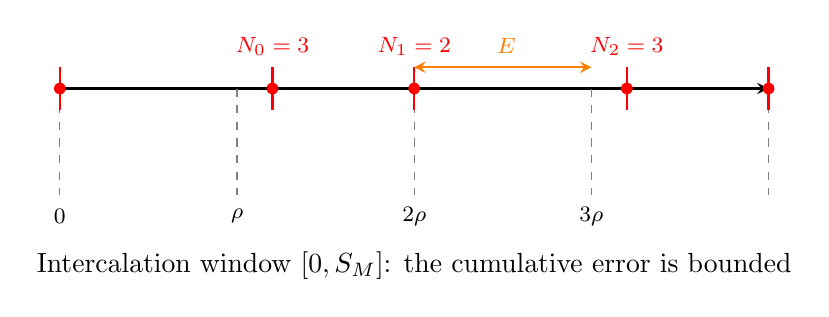
\begin{tikzpicture}[scale=0.9]
  % Ideal sampling positions
  \draw[->, thick, >=stealth] (0,0) -- (10,0);
  \foreach \x in {0,2.5,5,7.5,10} {
    \draw[gray, dashed] (\x,0) -- (\x,-1.5);
  }
  \node[font=\footnotesize] at (0,-1.8) {$0$};
  \node[font=\footnotesize] at (2.5,-1.8) {$\rho$};
  \node[font=\footnotesize] at (5,-1.8) {$2\rho$};
  \node[font=\footnotesize] at (7.5,-1.8) {$3\rho$};
  % Actual sampling positions (integers)
  \foreach \x in {0,3,5,8,10} {
    \draw[thick, red] (\x,0.3) -- (\x,-0.3);
    \node[circle, fill, red, inner sep=1.5pt] at (\x,0) {};
  }
  \node[red, font=\footnotesize] at (3,0.6) {$N_0=3$};
  \node[red, font=\footnotesize] at (5,0.6) {$N_1=2$};
  \node[red, font=\footnotesize] at (8,0.6) {$N_2=3$};
  % Error
  \draw[<->, thick, orange, >=stealth] (5,0.3) -- (7.5,0.3);
  \node[orange, font=\footnotesize] at (6.3,0.6) {$E$};
  \node at (5,-2.5) {Intercalation window $[0,S_M]$: the cumulative error is bounded};
\end{tikzpicture}
\caption{The intercalation sequence: the deviation between the ideal sampling positions (dashed lines) and the actual integer sampling positions (red dots) is confined within a bounded band.}
\label{fig:intercalation_error}
\end{figure}

\subsection{The Intercalation Functor}

\begin{definition}[Intercalation Functor]\label{def:intercalation_functor}
Let the sampling step $\Delta x>0$ and the intercalation mode (lower/upper/balanced) be fixed. Define the \textbf{intercalation functor}
\[
\mathcal{R}:\mathcal{C}_{\text{cont}}\to\mathcal{C}_{\text{trans}}
\]
by:
\begin{enumerate}[label=(\roman*)]
    \item \textbf{Object level}: for $F\in\mathcal{C}_{\text{cont}}$, set $\rho=\rho(F)$. If $\rho\in\mathbb{Q}$, let $\mathcal{R}(F)$ be any strict periodic extension of $\mathcal{D}(F)$ (well defined in $\mathcal{C}_{\text{trans}}$). If $\rho\notin\mathbb{Q}$, set
    \[
    \mathcal{R}(F)(n)=F(n\Delta x),\qquad n=0,1,\dots,S_M-1,\quad M\ \text{determined by the window},
    \]
    and take its $S_M$-periodic extension over the intercalation window in $\mathcal{C}_{\text{trans}}$.
    \item \textbf{Morphism level}: for a morphism $h:F\to G$ in $\mathcal{C}_{\text{cont}}$ (a linear map commuting with time translation), define $\mathcal{R}(h)$ as the linear map between the $S_M$-periodic sequences restricted to the intercalation window.
\end{enumerate}
\end{definition}

\begin{theorem}[Functoriality of the Intercalation Functor]\label{thm:intercalation_functoriality}
The intercalation functor $\mathcal{R}$ preserves identity morphisms and composition:
\begin{enumerate}[label=(\roman*)]
    \item $\mathcal{R}(\operatorname{id}_F)=\operatorname{id}_{\mathcal{R}(F)}$;
    \item for a composition $h_2\circ h_1$ in $\mathcal{C}_{\text{cont}}$, we have $\mathcal{R}(h_2\circ h_1)=\mathcal{R}(h_2)\circ\mathcal{R}(h_1)$.
\end{enumerate}
\end{theorem}

\begin{proof}
(i) The restriction of $\operatorname{id}_F$ to the sampling points $n\Delta x$ is the identity map, and after intercalation extension it remains the identity sequence.

(ii) Let $h_1:F\to G$ and $h_2:G\to K$ be morphisms in $\mathcal{C}_{\text{cont}}$. For any sampling point $n\Delta x$ ($n\in[0,S_M)$),
\[
[\mathcal{R}(h_2\circ h_1)](n)=(h_2\circ h_1)(F)(n\Delta x)=h_2(h_1(F(n\Delta x)))=[\mathcal{R}(h_2)\circ\mathcal{R}(h_1)](n).
\]
The pointwise equality on the intercalation window extends to an equality of $S_M$-periodic sequences, so $\mathcal{R}$ preserves composition.
\end{proof}

\begin{proposition}[Degeneracy in the Commensurable Case]\label{prop:intercalation_rational_degeneracy}
Let $F\in\mathcal{C}_{\text{cont}}$ be commensurable under $\Delta x$, that is, $\rho(F)=p/q\in\mathbb{Q}$ (in lowest terms). Then the intercalation functor degenerates to the discretisation functor: $\mathcal{R}(F)\cong\mathcal{D}(F)$, and $\operatorname{Group}_{\mathrm{period}}(\mathcal{R}(F))=p\mathbb{Z}$. In particular, the intercalation sequence is the constant sequence $N_m\equiv p$, and the intercalation error is identically zero.
\end{proposition}

\begin{proof}
By Proposition \ref{prop:commensurability_gap}(ii), $f(n)=F(n\Delta x)$ has period $p$. When the intercalation sequence is taken to be the constant sequence $N_m=p$, we have $S_M=Mp$, so $E(M)=Mp-Mp=0$. The intercalation-window extension coincides with the strict $p$-periodic extension of $\mathcal{D}(F)$. Hence $\mathcal{R}(F)\cong\mathcal{D}(F)$ and $\operatorname{Group}_{\mathrm{period}}(\mathcal{R}(F))=p\mathbb{Z}$.
\end{proof}

\begin{theorem}[Phase Correction of the Intercalation Functor]\label{thm:intercalation_phase_correction}
Let $F\in\mathcal{C}_{\text{cont}}$ be incommensurable, with $\rho=\rho(F)\notin\mathbb{Q}$, and let $\{N_m\}$ be the balanced intercalation sequence for $\rho$. Then for the continuous Fourier series $\displaystyle F(t)=\sum_{m\in\mathbb{Z}}c_m e^{i2\pi mt/T_F}$ on the intercalation window $[0,S_M]$, the $S_M$-point DFT of the sampling sequence $f(n)=F(n\Delta x)$ satisfies
\[
\hat{f}(k)=\sum_{m\in\mathbb{Z}}c_m\,D_{S_M}\!\left(\frac{m}{\rho}-\frac{k}{S_M}\right),
\]
where $D_T(\theta)=\dfrac{1}{T}\sum_{n=0}^{T-1}e^{i2\pi n\theta}$ is the Dirichlet kernel, and the main-lobe offset satisfies
\[
\left|\frac{m}{\rho}-\frac{k}{S_M}\right|\le\frac{|m|\,|E(M)|}{\rho\,S_M}\le\frac{|m|}{2\rho S_M}.
\]
That is, in the frequency domain the intercalation functor maps an incommensurable continuous object to a discrete object with \textbf{bounded phase error}---the phase error is controlled by the intercalation error $E(M)$.
\end{theorem}

\begin{proof}
Obtained directly from Theorem \ref{thm:intercalation_dft_leakage} of the `Harmonic Analysis' chapter (the DFT leakage estimate for the intercalation window), where balanced intercalation gives $|E(M)|\le 1/2$.
\end{proof}

\begin{corollary}[Phase Closure of the Intercalation Window]\label{cor:intercalation_window_closure}
Let $\rho\notin\mathbb{Q}$, and let $\{p_j/q_j\}$ be the continued-fraction convergents of $\rho$. Take $T=p_j$, $M=q_j$ (so that the intercalation window is $[0,p_j]$). Then the cumulative error within the intercalation window is
\[
|E(q_j)|=|p_j-q_j\rho|<\frac{1}{q_{j+1}},
\]
and the window approximately closes over $M=q_j$ continuous periods---when the intercalation functor $\mathcal{R}(F)$ is extended with period $S_M=p_j$ on the window $[0,p_j]$, the phase error is less than $1/q_{j+1}$.
\end{corollary}

\begin{proof}
Follows directly from Theorem \ref{thm:continued_fraction_best_approx_parallel} and Theorem \ref{thm:intercalation_phase_correction} of the `Discrete Sampling and Intercalation of Periodic Signals' chapter.
\end{proof}

\begin{theorem}[Universality of the Optimal Continued-Fraction Intercalation Functor]\label{thm:intercalation_continued_fraction}
Let $\rho>0$ be irrational, and let $\{p_j/q_j\}$ be its continued-fraction convergents. Then on the window sequence $\{(p_j,q_j)\}_{j\ge 0}$ above, the intercalation functor $\mathcal{R}$ satisfies
\[
\lim_{j\to\infty}\frac{|E(q_j)|}{p_j}=0,\qquad
\frac{|E(q_j)|}{p_j}<\frac{1}{p_j q_{j+1}}\to 0.
\]
That is, along the continued-fraction convergent window sequence the \textbf{relative phase error} of the intercalation functor $\mathcal{R}$ tends to zero---in the limiting sense the intercalation functor \textbf{restores} the categorical connection between $\mathcal{C}_{\text{cont}}$ and $\mathcal{C}_{\text{trans}}$ that was severed by the commensurability gap.
\end{theorem}

\begin{proof}
From the main-lobe offset bound $|m|\,|E|/(\rho S_M)$ of Theorem \ref{thm:intercalation_phase_correction} and the bound $|E(q_j)|<1/q_{j+1}$ of Corollary \ref{cor:intercalation_window_closure}, we obtain
\[
\frac{|E(q_j)|}{p_j}<\frac{1}{p_j q_{j+1}}.
\]
By the theory of continued fractions, $p_j,q_j\to\infty$ and $q_{j+1}>q_j$, so $1/(p_j q_{j+1})\to 0$.
\end{proof}

\subsection{Commutation of the Intercalation Functor and the Continuum-Limit Functor}

\begin{theorem}[Commutation of the Intercalation Functor and the Continuum-Limit Functor]\label{thm:intercalation_continuum_commutation}
Let $\mathcal{D}:\mathbf{Man}\to\mathbf{Latt}$ be the discretisation functor, $\mathcal{C}_\infty:\mathbf{Latt}\to\mathbf{Man}$ the continuum-limit functor (defined in the preceding section, \ref{def:continuum_limit_functor}), and $\mathcal{R}:\mathcal{C}_{\text{cont}}\to\mathcal{C}_{\text{trans}}$ the intercalation functor. Then the following diagram commutes in the limiting sense:
\[
\begin{tikzcd}[row sep=large, column sep=large]
\mathcal{C}_{\text{cont}} \arrow[r, "\mathcal{R}"] \arrow[d, "\text{embedding}"'] & \mathcal{C}_{\text{trans}} \arrow[d, "\mathcal{D}"] \\
\mathbf{Man} \arrow[r, "\mathcal{C}_\infty"'] & \mathbf{Latt}
\end{tikzcd}
\]
More precisely: for $F\in\mathcal{C}_{\text{cont}}$, take the sequence of intercalation windows $\{(p_j,q_j)\}_{j\ge 0}$ (with $p_j\to\infty$). Then
\[
\lim_{j\to\infty}\mathcal{D}\big(\mathcal{R}_j(F)\big)=\mathcal{D}\big(\mathcal{D}(F)\big),
\]
where $\mathcal{R}_j$ denotes the intercalation functor on the $j$-th intercalation window, and $\mathcal{D}(\mathcal{R}_j(F))$ is the realisation of the intercalation sequence on the lattice points.
\end{theorem}

\begin{proof}
By Theorem \ref{thm:intercalation_continued_fraction}, on the $j$-th window the relative phase error of the intercalation sequence $\mathcal{R}_j(F)$ tends to zero. Hence on the window $[0,p_j]$, the difference between $\mathcal{R}_j(F)$ and $\mathcal{D}(F)$ tends to zero in the sense of bounded error. Letting $j\to\infty$, the two discrete sequences converge to the same object in the lattice category.
\end{proof}

\begin{remark}[The Categorical Status of the Intercalation Functor]\label{rem:intercalation_category_status}
The relation between the intercalation functor $\mathcal{R}$ and the discretisation functor $\mathcal{D}$ may be understood as follows: $\mathcal{R}$ is a \textbf{bounded-error correction} of $\mathcal{D}$ in the incommensurable case. When $\rho\in\mathbb{Q}$ the two are isomorphic (Proposition \ref{prop:intercalation_rational_degeneracy}); when $\rho\notin\mathbb{Q}$, $\mathcal{R}$ drives the phase error to zero by choosing continued-fraction convergence windows (Theorem \ref{thm:intercalation_continued_fraction}), thereby restoring the categorical nature of $\mathcal{D}$ in the limiting sense.

From the perspective of adjoint functors, if the discretisation functor $\mathcal{D}$ is regarded as the left adjoint and the continuum-limit functor $\mathcal{C}_\infty$ as the right adjoint (Proposition \ref{prop:continuum_limit_adjunction} of the preceding section), then the intercalation functor $\mathcal{R}$ may be regarded as a \textbf{consistency correction} of the adjoint pair $(\mathcal{D},\mathcal{C}_\infty)$ in the incommensurable case---it does not change the adjoint pair itself, but carries correction data at the level of objects, so that the natural isomorphism of the adjunction is preserved to arbitrary precision in the incommensurable case.
\end{remark}

\begin{proposition}[Conserved Quantities of the Intercalation Functor]\label{prop:intercalation_conservation}
At the level of objects, the intercalation functor $\mathcal{R}$ carries the following conserved quantities:
\begin{enumerate}[label=(\roman*)]
    \item \textbf{Boundedness of the cumulative error}: $|E(M)|\le C$ holds for all $M$---the phase error of the intercalation sequence is conserved and bounded on the scale of the window;
    \item \textbf{Monotone convergence of the relative error}: $\displaystyle\lim_{j\to\infty}\frac{|E(q_j)|}{p_j}=0$---the relative phase error on the continued-fraction convergence windows tends to zero;
    \item \textbf{Conservation of energy}: the DFT Parseval identity on the intercalation window
    \[
    \sum_{n=0}^{S_M-1}|f(n)|^2=S_M\sum_{k=0}^{S_M-1}|\hat{f}(k)|^2
    \]
    holds exactly on the intercalation window---intercalation does not change the total energy within the window.
\end{enumerate}
\end{proposition}

\begin{proof}
(i) By Lemma \ref{lem:intercalation_error_bound_category}. (ii) By Theorem \ref{thm:intercalation_continued_fraction}. (iii) By applying Theorem \ref{thm:discrete_parseval_parallel} of the `Discrete Sampling and Intercalation of Periodic Signals' chapter on the intercalation window.
\end{proof}

\begin{remark}[The Interface between the Intercalation Functor and the Observer Functor]\label{rem:intercalation_observer_interface}
The relation between the intercalation functor $\mathcal{R}$ and the observer functor $\mathcal{P}$ (defined in the next section, \ref{def:observer_functor}) is as follows: the observer functor extracts observable traces, whilst the intercalation functor determines the optimal length of the observer's sampling window. Concretely, the intercalation functor gives the window sequence $\{(p_j,q_j)\}$, and the observer functor projects observable traces onto this window---intercalation makes the observer's sampling window approximately contain an integer number of continuous periods, thereby minimising the phase error of the projection. Together the two form a `sampling--projection' double functor
\[
\mathcal{C}_{\text{cont}}\xrightarrow{\mathcal{R}}\mathcal{C}_{\text{trans}}\xrightarrow{\mathcal{P}}\mathcal{C}_{\text{obs}},
\]
where $\mathcal{R}$ renders the phase error bounded and $\mathcal{P}$ renders the structural projection conformal.
\end{remark}

\begin{figure}[htbp]
\centering
\begin{tikzcd}[row sep=large, column sep=large]
\mathcal{C}_{\text{cont}} \arrow[r, "\mathcal{R}"] \arrow[d, "\text{embedding}"'] & \mathcal{C}_{\text{trans}} \arrow[d, "\mathcal{D}"] \\
\mathbf{Man} \arrow[r, "\mathcal{C}_\infty"'] & \mathbf{Latt}
\end{tikzcd}
\caption{Commutative diagram of the intercalation functor and the continuum-limit functor: they commute in the limiting sense.}
\label{fig:intercalation_commutation}
\end{figure}

\section{The Observer as a Functor}\label{sec:observer_functor}

\begin{definition}[The Observer Functor]\label{def:observer_functor}
The \textbf{observer functor} $\mathcal{P}: \mathcal{C}_{\text{trans}} \times \mathcal{C}_{\text{rot}} \to \mathcal{C}_{\text{obs}}$ maps the product of the time-periodic category and the rotation-periodic category to the \textbf{category of observable traces} $\mathcal{C}_{\text{obs}}$:
\[
\mathcal{P}(f_T, f_S) = \mathcal{N}(r, \sigma) \cdot \left( \Phi(f_T) \cdot \nabla S + \Phi(f_S) \cdot \nabla S \right) \cdot \mathbf{u}_P,
\]
where $\mathcal{N}(r, \sigma) = (\sigma/(r^2+\sigma))^2$ is the sampling normalisation factor, $\Phi$ is the phase-extraction functor, and $\mathbf{u}_P$ is the line-of-sight direction of the observer.
\end{definition}

\begin{theorem}[Decomposition of the Observer Functor]\label{thm:observer_functor_decomposition}
The observer functor $\mathcal{P}$ can be decomposed as the composition of three sub-functors:
\[
\mathcal{P} = \mathcal{P}_{\cdot} \circ \operatorname{add} \circ (\mathcal{P}_{\nabla} \times \mathcal{P}_{\times}),
\]
where $\mathcal{P}_{\nabla}$ projects the temporal flux onto the irrotational part of the observable field, $\mathcal{P}_{\times}$ projects the spatial flux onto the solenoidal part, and $\mathcal{P}_{\cdot}$ applies the normalisation factor.
\end{theorem}

\begin{proof}
This follows by decomposing term by term the explicit formula of Definition \ref{def:observer_functor}. The irrotational/solenoidal decomposition is guaranteed by the Helmholtz decomposition theorem of the `Vector Analysis' chapter (Theorem \ref{thm:helmholtz}).
\end{proof}

\begin{corollary}[The Observer Functor and Adjunction]\label{cor:observer_adjunction}
The observer functor $\mathcal{P}$ has a left adjoint $\mathcal{P}^*$ (the reconstruction functor), forming an adjoint pair:
\[
\mathcal{P}^* \dashv \mathcal{P}.
\]
The unit $\eta$ of the adjunction is not an isomorphism---the loss of information in the process of observation is irreversible.
\end{corollary}

\begin{proof}
Construct $\mathcal{P}^*$ as the canonical lift: for each trace $O$, take $\mathcal{P}^*(O)$ to be the minimal-norm preimage satisfying $\mathcal{P}(\mathcal{P}^*(O)) = O$. The adjunction bijection is given by the linear structure. The unit $\eta$ is not an isomorphism because the canonical lift is not a section of the observation.
\end{proof}

\begin{remark}[The Observer Functor and the Breaking of Conservation Laws]\label{rem:observer_conservation_breaking}
The unit $\eta$ of the adjunction not being an isomorphism means that the observer cannot completely reconstruct the original periodic structure from the observable traces. The loss of information in the process of observation is irreversible---the conserved quantities of the time system and the space system (energy, angular momentum) are partially destroyed by the divergence of the observing system (symmetry centre $1$) (sampling decay, projection selection).
\end{remark}

\begin{figure}[htbp]
\centering
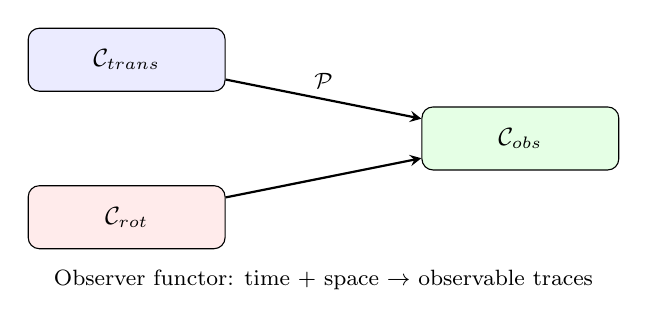
\begin{tikzpicture}[font=\small, arr/.style={->, thick, >=stealth}]
  \node[draw, rounded corners, fill=blue!8, minimum width=2.5cm, minimum height=0.8cm] (T) at (0,1) {$\mathcal C_{\text{trans}}$};
  \node[draw, rounded corners, fill=red!8, minimum width=2.5cm, minimum height=0.8cm] (R) at (0,-1) {$\mathcal C_{\text{rot}}$};
  \node[draw, rounded corners, fill=green!10, minimum width=2.5cm, minimum height=0.8cm] (O) at (5,0) {$\mathcal C_{\text{obs}}$};
  \draw[arr] (T) -- node[above, font=\footnotesize]{$\mathcal P$} (O);
  \draw[arr] (R) -- (O);
  \node[font=\footnotesize] at (2.5,-1.8) {Observer functor: time + space $\to$ observable traces};
\end{tikzpicture}
\caption{The observer functor $\mathcal{P}$: it projects the product of the time-periodic category and the rotation-periodic category onto the category of observable traces.}
\label{fig:observer_functor}
\end{figure}

\section{Periodic Categories and Conservation Laws}\label{sec:periodic_category_conservation_laws}

\begin{theorem}[A Categorical Formulation of Noether's Theorem]\label{thm:noether_categorical}
Let $\mathcal{C}^G$ be a $G$-periodic category, where $G$ is a Lie group. There exists a natural isomorphism:
\[
\operatorname{Symmetry}(\mathcal{C}^G) \cong \operatorname{Conserved}(\mathcal{C}^G),
\]
where $\operatorname{Symmetry}(\mathcal{C}^G)$ is the group of continuous symmetries of $\mathcal{C}^G$ and $\operatorname{Conserved}(\mathcal{C}^G)$ is the space of conserved quantities of $\mathcal{C}^G$.

Specifically:
\begin{enumerate}[label=(\roman*)]
    \item Translational symmetry ($G = \mathbb{R}$, $0$-symmetry) $\cong$ conservation of energy/momentum.
    \item Rotational symmetry ($G = U(1)$, $i$-symmetry) $\cong$ conservation of angular momentum.
    \item Scaling symmetry ($G = \mathbb{R}^+$, $1$-symmetry) $\cong$ conservation of the scale charge.
\end{enumerate}
\end{theorem}

\begin{proof}
For each object $(X, \rho) \in \mathcal{C}^G$: every one-parameter subgroup of $G$, through the action $\rho$, gives a one-parameter family of automorphisms of $X$, whose infinitesimal generator corresponds to the Noether charge, namely the conserved quantity (Theorem \ref{thm:noether_group_with_periodic_orbits} of the `Periodic Functions and Groups with Periodic Orbits' chapter). Naturality is given by the equivariance of periodic morphisms.
\end{proof}

\begin{figure}[htbp]
\centering
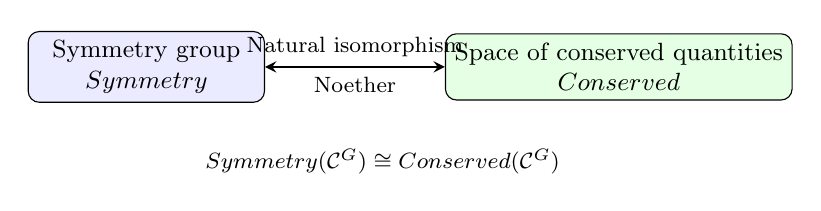
\begin{tikzpicture}[font=\small, arr/.style={->, thick, >=stealth}]
  \node[draw, rounded corners, fill=blue!8, minimum width=3cm, minimum height=0.8cm, align=center] (sym) {Symmetry group\\$\operatorname{Symmetry}$};
  \node[draw, rounded corners, fill=green!10, minimum width=3cm, minimum height=0.8cm, align=center] (cons) at (6,0) {Space of conserved quantities\\$\operatorname{Conserved}$};
  \draw[<->, thick, >=stealth] (sym) -- node[above, font=\footnotesize]{Natural isomorphism} node[below, font=\footnotesize]{Noether} (cons);
  \node[font=\footnotesize] at (3,-1.2) {$\operatorname{Symmetry}(\mathcal C^G)\cong\operatorname{Conserved}(\mathcal C^G)$};
\end{tikzpicture}
\caption{A categorical formulation of Noether's theorem: the natural isomorphism between the symmetry group and the space of conserved quantities.}
\label{fig:noether_categorical}
\end{figure}

\section{A Unified Perspective on Periodic Categories}\label{sec:periodic_category_unification}

\begin{theorem}[The Categorical Unification of Periodic Mathematics]\label{thm:periodic_category_unification}
The core structures of periodic mathematics can be unified through the following commutative diagram:
\[
\begin{tikzcd}
\mathcal{C}_{\text{scal}} \arrow[r, "\mathcal{L}"] \arrow[d, "\mathcal{F}_{\text{scal}}"'] & \mathcal{C}_{\text{trans}} \arrow[d, "\mathcal{F}_{\text{trans}}"] \\
\mathbf{Vect}_{\mathbb{C}} \arrow[r, "\mathcal{L}_*"'] & \mathbf{Vect}_{\mathbb{C}}
\end{tikzcd}
\]
where $\mathcal{L}$ is the logarithm functor, $\mathcal{F}_{\text{trans}}$ is the Fourier transform and $\mathcal{F}_{\text{scal}}$ is the Mellin transform. The commutativity of the left-hand square is verified directly by the substitution $x = e^t$.
\end{theorem}

\begin{proof}
Under the substitution $x = e^t$, the scaling-periodic function $f(x)$ becomes the translation-periodic function $g(t) = f(e^t)$. The Mellin transform $\mathcal{F}_{\text{scal}}$ and the Fourier transform $\mathcal{F}_{\text{trans}}$ commute under this substitution: $\mathcal{F}_{\text{trans}}(\mathcal{L}f) = \mathcal{L}_*(\mathcal{F}_{\text{scal}}f)$. The conservation structure is guaranteed by Theorem \ref{thm:noether_categorical} and the Parseval identity.
\end{proof}

\begin{remark}[The Pivotal Role of Periodic Categories throughout the Book]\label{rem:periodic_category_hub}
The periodic category is the highest level of abstraction in the theoretical system of periodic mathematics. It brings into the language of category theory the group-representation prototypes of the `Operations and Periodicity' chapter, the centres of symmetry of the `Number Systems' chapter, the similarity and tendency of the `Scalars and Vectors' chapter, the calculus foundations of the `Functions and Limits' chapter, the periodic transforms and convolutions of the `Series and Convolution' chapter, and the discrete geometry of the `Periodic Manifold' chapter---all unified together.

Within this unified framework:
\begin{itemize}
    \item \textbf{Period} is the natural expression, at the level of category theory, of invariance under a group action---the $G$-periodic object $(X, \rho)$.
    \item \textbf{Conservation laws} are the natural isomorphism, at the level of functors, of the Noether charges of continuous symmetries---$\operatorname{Symmetry} \cong \operatorname{Conserved}$.
    \item \textbf{Phase} is a structure-preserving map on a category---any phase of any period may serve as a functor (Corollary \ref{cor:all_phases_functorial}).
    \item \textbf{Differentiation and integration} are an adjoint pair of operators on the periodic category---$\mathcal{D} \dashv \mathcal{I}$.
    \item \textbf{Convolution and periodic convolution} are bifunctors on the periodic category---$*$ and $\circledast$.
    \item \textbf{The observer} is the central functor connecting the time system and the space system---$\mathcal{P}$.
\end{itemize}
\end{remark}

\begin{remark}[An Outlook on Higher Categories]\label{ch13_higher_category_remark}
This chapter takes the natural transformation (Definition \ref{def:natural_transformation}) as the highest-level structure. A natural next step is to incorporate into the framework the morphisms between natural transformations---modifications: the continuous variation of a family of periodic parameters is precisely an instance of a modification, and in this case the periodic category organises into a $2$-category. The fact that the adjunction unit of the observer functor is not an isomorphism shows that the observation--reconstruction cycle forms an irreversible $2$-morphism at the level of the $2$-category. This is a prospective note, and no theorem is established.
\end{remark}

\section*{Seven-theme comparison table for this chapter}

\begin{figure}[htbp]
\centering
\begin{tikzpicture}[
  theme/.style={draw, rounded corners, fill=green!10, minimum width=1.2cm, minimum height=0.55cm, align=center, font=\footnotesize}
]
  \node[theme] (p) at (0,0) {Translation};
  \node[theme, right=0.3cm of p] (s) {Scaling};
  \node[theme, right=0.3cm of s] (r) {Rotation};
  \node[theme, right=0.3cm of r] (c) {Conservation};
  \node[theme, right=0.3cm of c] (sym) {Symmetry};
  \node[theme, right=0.3cm of sym] (cl) {Closure};
  \node[theme, right=0.3cm of cl] (per) {Period};
  \node[draw, dashed, rounded corners, fit=(p)(per), inner sep=6pt] (box) {};
  \node[below=0.1cm of box, font=\footnotesize] {Seven themes running through periodic categories};
\end{tikzpicture}
\caption{The seven themes of this chapter: translation, scaling, rotation, conservation, symmetry, closure and period.}
\label{fig:periodic_category_themes}
\end{figure}

\begin{center}
\begin{tabular}{>{\centering\arraybackslash}p{2.2cm}>{\centering\arraybackslash}p{10.5cm}}
\toprule
Theme & Corresponding content in this chapter \\
\midrule
Translation & The translation-periodic category $\mathcal{C}_{\text{trans}}$ and the differential operator $\mathcal{D}$ ($0$-symmetry); the cumulative sample count $S_M$ of the intercalation sequence approximates $M\rho$ (Definition \ref{def:intercalation_object}) \\
Scaling & The scaling-periodic category and the logarithm/exponential functors ($1$-symmetry); the ideal period ratio $\rho$ as the scale charge (Definition \ref{def:ideal_period_ratio_categorical}) \\
Rotation & The rotation-periodic category, the phase functor and the Fourier functor ($i$-symmetry); the phase correction of the intercalation window (Theorem \ref{thm:intercalation_phase_correction}) \\
Conservation & The conservation condition for adjoint operators (Corollary \ref{cor:diff_int_conservation}); the categorical formulation of Noether's theorem (Theorem \ref{thm:noether_categorical}); the boundedness of the cumulative intercalation error (Lemma \ref{lem:intercalation_error_bound_category}) \\
Symmetry & Natural isomorphism and the adjoint duality $\mathcal{D}\dashv\mathcal{I}$; the family of phase functors $\cong U(1)$ (Theorem \ref{thm:phase_functor_group}); the symmetric approximation by continued-fraction convergents (Theorem \ref{thm:intercalation_continued_fraction}) \\
Closure & The mutual-inverse closure of the differential and integral operators (Lemma \ref{ch13_diff_int_inverse_lemma}); the closure property of the periodic-convolution bifunctor (Theorem \ref{thm:periodic_convolution_functoriality}); the intercalation window closes the approximate period (Corollary \ref{cor:intercalation_window_closure}) \\
Period & The categorical formulation of periodic manifolds; the parametrisation of the phase functor (Corollary \ref{cor:all_phases_functorial}); when $\rho\in\mathbb{Q}$ the intercalation functor degenerates to a strict periodic functor (Proposition \ref{prop:intercalation_rational_degeneracy}) \\
\bottomrule
\end{tabular}
\end{center}

\section*{Exercises}

\begin{enumerate}[leftmargin=3em, label=\textbf{Exercise \arabic*}]
    \item Using Definition \ref{def:operator} and Definition \ref{def:functor},
    explain the essential difference in scope between an operator (endofunctor) and a functor.
    Give one example of each: an operator that leaves the periodic type unchanged,
    and a functor that maps the translation-periodic category to another category (for instance the Fourier functor, which maps periodic functions to sequences of Fourier coefficients).

    \item Prove the six basic properties of the phase functor
    $\Phi_{\theta,T}$ in Proposition \ref{prop:phase_functor_properties}:
    functoriality, period preservation, the composition law, the identity element, the inverse element and unitarity.
    Also verify Theorem \ref{thm:phase_functor_group}:
    the family of phase functors for a fixed period $T$ forms a group under composition, isomorphic to $U(1)$.

    \item Verify the concrete action of the phase functor on the sine function in Example \ref{ex:phase_functor_action}:
    take $T=2\pi$ and $f(t)=\sin t$, and compute
    \[
    \Phi_{\pi/2,2\pi}(f)(t),\qquad
    \Phi_{\pi,2\pi}(f)(t).
    \]
    Explain why $\Phi_{\pi,2\pi}$ is the identity map on the sine function,
    and point out how this is related to the antipodal relation when the phase is $\pi$.

    \item Prove Lemma \ref{ch13_hom_frequency_lemma}:
    let $f(t)=Ae^{i(\omega_1t+\varphi)}$ and $g(t)=Be^{i(\omega_2t+\psi)}$ be two single-frequency circle objects.
    \begin{enumerate}[label=(\roman*)]
        \item If $\omega_1\neq\omega_2$, then $\operatorname{Hom}(f,g)=\{0\}$;
        \item If $\omega_1=\omega_2=\omega$, then
              $\operatorname{Hom}(f,g)=\{c\cdot\frac{B}{A}e^{i(\psi-\varphi)}:c\in\mathbb{C}\}$.
    \end{enumerate}
    Explain why amplitude and phase are not invariants of the translation-periodic category
    (see Remark \ref{ch13_amplitude_phase_remark}).

    \item Verify the computation of the morphisms between the three single-frequency circle objects in Example \ref{ch13_hom_set_example}:
    \[
    f(t)=3e^{i(2t+\pi/6)},\quad
    g(t)=2e^{i(3t-\pi/4)},\quad
    h(t)=5e^{i(2t+\pi/3)}.
    \]
    Compute $\operatorname{Hom}(f,g)$, $\operatorname{Hom}(f,h)$ and $\operatorname{Hom}(h,k)$ (taking $k(t)=4e^{i2t}$),
    and verify the composition law $\mu\circ\lambda=\nu$.

    \item Prove Theorem \ref{thm:diff_int_adjunction}:
    on the translation-periodic category, the differential operator $\mathcal{D}$ and the integral operator $\mathcal{I}$
    form the adjoint pair $\mathcal{D}\dashv\mathcal{I}$.
    Write down the natural isomorphism of the adjunction, and explain why the zero-mean condition is needed.

    \item Verify Lemma \ref{ch13_diff_int_inverse_lemma}:
    \[
    (\mathcal{D}\circ\mathcal{I})(f)=f-\bar{f},\qquad
    (\mathcal{I}\circ\mathcal{D})(f)=f-f(0).
    \]
    On the quotient category (modulo constants) of zero-mean periodic functions, the two are mutually strict inverses.
    Verify this with the numerical example \ref{ch13_adjunction_numeric_example}.

    \item Prove Proposition \ref{prop:three_category_functors}:
    there exist natural functors among the three periodic categories---
    the logarithm functor $\mathcal{L}:\mathcal{C}_{\text{scal}}\to\mathcal{C}_{\text{trans}}$,
    the exponential functor $\mathcal{E}:\mathcal{C}_{\text{trans}}\to\mathcal{C}_{\text{scal}}$,
    and the Fourier functor $\mathcal{F}:\mathcal{C}_{\text{trans}}\to\mathbf{Vect}_{\mathbb{C}}$.
    Also prove Corollary \ref{cor:grammar_adjunction}: $\mathcal{L}\dashv\mathcal{E}$.

    \item Prove Theorem \ref{thm:periodic_convolution_functoriality_series}:
    the periodic convolution $\circledast$ is a bifunctor on the translation-periodic category, satisfying
    preservation of identities, preservation of composition, compatibility with the similarity functor, and compatibility with the tendency functor.
    Explain that periodic convolution is represented in the frequency domain by the tensor product, and that phase and tendency are represented in the frequency domain by pointwise operations.

    \item Prove Proposition \ref{prop:commensurability_gap}:
    the commensurability gap---when $\rho=T_F/\Delta x\in\mathbb{Q}$,
    the discretisation functor $\mathcal{D}$ preserves the periodic structure;
    when $\rho\notin\mathbb{Q}$, $\mathcal{D}$ fails to preserve the periodic structure on $F$.
    Discuss the three cases $\rho\in\mathbb{N}^+$, $\rho\in\mathbb{Q}\setminus\mathbb{N}^+$ and $\rho\notin\mathbb{Q}$ separately.

    \item Prove Theorem \ref{thm:intercalation_functoriality}:
    the intercalation functor $\mathcal{R}$ preserves identity morphisms and composition.
    Explain why the intercalation functor is a bounded-error correction of the discretisation functor $\mathcal{D}$ in the incommensurable case
    (see Remark \ref{rem:intercalation_category_status}).

    \item Prove Theorem \ref{thm:intercalation_phase_correction}:
    in the frequency domain, the intercalation functor maps an incommensurable continuous object to a discrete object with bounded phase error.
    Write down the bound on the main-lobe offset
    \[
    \left|\frac{m}{\rho}-\frac{k}{S_M}\right|
    \le\frac{|m|\,|E(M)|}{\rho\,S_M}\le\frac{|m|}{2\rho S_M},
    \]
    and explain that balanced intercalation gives $|E(M)|\le1/2$.

    \item Prove Theorem \ref{thm:intercalation_continuum_commutation}:
    the intercalation functor and the continuum-limit functor commute in the limiting sense.
    Write down the commutative diagram, and explain why the relative phase error tends to zero along the continued-fraction convergence window sequence
    (see Theorem \ref{thm:intercalation_continued_fraction}).

    \item Verify the three conserved quantities of the intercalation functor in Proposition \ref{prop:intercalation_conservation}:
    boundedness of the cumulative error, monotone convergence of the relative error, and conservation of energy.
    Taking $\rho=\sqrt{2}$ as an example, compute the relative errors corresponding to
    the continued-fraction denominator sequence $q_k=1,2,5,12,29,70,\dots$.

    \item Prove Proposition \ref{prop:three_convolutions_relation}:
    \begin{enumerate}[label=(\roman*)]
        \item the trend convolution $=$ the amplitude convolution $\times$ the phase convolution;
        \item the frequency convolution $=$ the outer product of frequency series;
        \item the three capture, in the frequency domain, the three independent components of convolution---amplitude, phase and frequency.
    \end{enumerate}

    \item Verify Proposition \ref{prop:periodic_convolution_hierarchy}:
    the periodic convolution is the summit of the five-level ladder of convolution theory:
    \[
    \text{periodic convolution}\circledast\to
    \text{trend convolution}\mathbb{T}\to
    \text{classical convolution}*.
    \]
    Write down the concrete forms of the degeneration at the single-period level and of the diagonal-kernel degeneration,
    and explain that the information content of each step of the ladder is strictly increasing.

    \item Prove Theorem \ref{thm:noether_categorical}:
    the categorical formulation of Noether's theorem---
    there exists a natural isomorphism
    \[
    \operatorname{Symmetry}(\mathcal{C}^G)\cong\operatorname{Conserved}(\mathcal{C}^G).
    \]
    Write out the three cases separately: translational symmetry (corresponding to conservation of energy/momentum),
    rotational symmetry (corresponding to conservation of angular momentum),
    and scaling symmetry (corresponding to conservation of the scale charge).

    \item Verify the commutative diagram in Theorem \ref{thm:periodic_category_unification}:
    \[
    \begin{tikzcd}
    \mathcal{C}_{\text{scal}} \arrow[r,"\mathcal{L}"] \arrow[d,"\mathcal{F}_{\text{scal}}"']
    & \mathcal{C}_{\text{trans}} \arrow[d,"\mathcal{F}_{\text{trans}}"] \\
    \mathbf{Vect}_{\mathbb{C}} \arrow[r,"\mathcal{L}_*"']
    & \mathbf{Vect}_{\mathbb{C}}
    \end{tikzcd}
    \]
    Explain that the commutativity of the left-hand square is verified directly by the substitution $x=e^t$,
    and point out the correspondence between the Mellin transform and the Fourier transform under this substitution.

    \item Comprehensive question: combining the phase functor (Definition \ref{def:phase_functor_general}),
    the similarity and tendency functors (Definitions \ref{def:similarity_functor}, \ref{def:tendency_functor}),
    the differentiation--integration adjunction (Theorem \ref{thm:diff_int_adjunction}),
    the periodic-convolution bifunctor (Definition \ref{def:periodic_convolution_bifunctor})
    and the observer functor (Definition \ref{def:observer_functor}),
    explain how the periodic category unifies the theoretical structure of the whole book within the language of category theory.
    Point out separately the categorical objects corresponding to `period', `conservation laws', `phase', `differentiation and integration', `convolution' and `the observer'
    in the periodic category.
\end{enumerate}
